\documentclass[11pt]{article}

\usepackage[letterpaper,margin=1in]{geometry}
\usepackage[T1]{fontenc}
\usepackage{amsmath,amsthm}
\usepackage{stix2}
\usepackage[varqu,scaled=0.95]{zi4}
\usepackage{graphicx}
\usepackage{booktabs}
\usepackage{array}
\usepackage{listings}
\usepackage[font=small,list=no]{caption}
\captionsetup[lstlisting]{singlelinecheck=false}
\usepackage{enumitem}
\usepackage{microtype}
\usepackage{needspace}
\usepackage[hidelinks,pdftitle={Conley indices of Morse sets on adaptive grids in CMGDB},pdfauthor={Bernardo Rivas}]{hyperref}

\graphicspath{{figures/}}
\renewcommand{\topfraction}{0.9}
\renewcommand{\bottomfraction}{0.6}
\renewcommand{\textfraction}{0.08}
\renewcommand{\floatpagefraction}{0.8}
\setlength{\emergencystretch}{3em}
\renewcommand{\UrlBreaks}{\do\/\do\_\do\.\do\-}

\theoremstyle{plain}
\newtheorem{proposition}{Proposition}[section]
\newtheorem{lemma}[proposition]{Lemma}
\newtheorem{corollary}[proposition]{Corollary}
\theoremstyle{definition}
\newtheorem{definition}[proposition]{Definition}
\newtheorem{example}[proposition]{Example}
\theoremstyle{remark}
\newtheorem{remark}[proposition]{Remark}

\DeclareMathOperator{\Inv}{Inv}
\DeclareMathOperator{\cover}{cover}
\DeclareMathOperator{\hull}{hull}
\DeclareMathOperator{\depth}{depth}
\DeclareMathOperator{\cl}{cl}
\DeclareMathOperator{\interior}{int}
\DeclareMathOperator{\sign}{sign}
\DeclareMathOperator{\CH}{CH}
\newcommand{\F}{\mathbb{F}_5}
\newcommand{\R}{\mathbb{R}}
\newcommand{\Fc}{\mathcal{F}}
\newcommand{\Ft}{\tilde{\mathcal{F}}}
\newcommand{\lo}{\mathrm{lo}}
\newcommand{\hi}{\mathrm{hi}}
\newcommand{\dmin}{d_{\min}}
\newcommand{\dmax}{d_{\max}}
\newcommand{\dinit}{d_{\mathrm{init}}}
\newcommand{\Phipad}{\Phi_{\mathrm{pad}}}
\newcommand{\Phihull}{\Phi_{\mathrm{hull}}}
\newcommand{\code}[1]{\texttt{#1}}
\newcommand{\undefidx}{[\,]}

\lstdefinestyle{report}{basicstyle=\ttfamily\small,columns=fullflexible,keepspaces=true,frame=lines,framesep=4pt,numbers=left,numberstyle=\scriptsize\ttfamily,numbersep=8pt,xleftmargin=2.2em,upquote=true,showstringspaces=false,keywordstyle={},commentstyle={},stringstyle={},identifierstyle={}}
\lstset{style=report}

\title{Conley indices of Morse sets on adaptive grids in CMGDB}
\author{Bernardo Rivas}
\date{October 6, 2026}

\begin{document}

\maketitle

\begin{center}
\small Code baseline: the fork \code{bernardorivas/CMGDB} at master 96642f2. Builds before the changes: upstream CMGDB 1.5.2, the fork release 1.3.3+fork.6, and the merge 0e21503 of upstream 1.5.2 into the fork, before the fixes.
\end{center}

\section{Summary}\label{sec:summary}

CMGDB computes the Conley index of a Morse set $S$ of the final grid from the pair $X=\cover F(S)$, $A=X\setminus S$ of cells, converted into a pair of cubical sets at the depth of $S$. On the grids of the adaptive hierarchy, two separate defects make the result differ from the Conley index of the invariant set in $|S|$.

The first defect lies in the coordinates of the cubical complex (Part I, Section~\ref{sec:c43}). A cell of $X$ deeper than $S$ enters the complex as its ancestor at the depth of $S$, but the code bounded the complex by the hull of the cells of $X$, which can stop short of such an ancestor. The coordinates of the cubes divide the bounds evenly, so the box map $F$ was evaluated on boxes that are not cells, and the map on cubes was that of $\varphi^{-1}\circ F\circ\varphi$ for an affine map $\varphi$, which is $\varphi^{-1}\circ f\circ\varphi$ for the box maps of Part I (Proposition~\ref{prop:old}). For this map the cubical pair can fail to be an index pair, and it does in the examples E1 to E5 of Section~\ref{sec:examples}, where hyperbolic fixed points received trivial or undefined indices and \code{ComputeConleyMorseGraph} of the fork release 1.3.3+fork.6 raised an exception (Table~\ref{tab:annotations}). The defect needs $\dmax>\dmin$, where $\dmin$ is the depth of the Morse sets and $\dmax$ the largest depth of the hierarchy (Section~\ref{sec:hierarchy}). Commit 577d988, ``Bound the relative complex by the cubes it holds'', bounds the complex by its cubes, and master 96642f2 returns the index of the linearization at every fixed point of the examples.

The second defect lies in the hierarchy (Part II, Section~\ref{sec:leslie}). With a box map that is not monotone under refinement, such as the box $\Phi(B)$ spanned by $f$ at the corners of a box $B$, the hierarchy can leave a coarse cell unrefined although it lies on a cycle through a Morse set of the final grid. The pair of that Morse set is then not an index pair, and its annotation can differ from that of the Conley index of the invariant set. For the Leslie map, the Morse set around the repelling focus in the run $12/14$ with $\Phi$, which has $\dmin=12$ and $\dmax=14$, is annotated $(0,x+1,0)$. Its invariant set is an attractor whose index has the annotation $(x-1,0,0)$, which the run $16/18$ with $\Phi$ returns (Proposition~\ref{prop:isolation}, which rests on a computation with explicit margins). This defect is present on every build, including master. Since commit 86b143a, \code{ComputeConleyIndexForCells} refuses such a set with \code{ValueError}, but \code{ComputeConleyMorseGraph} still annotates it, and no warning has been implemented. If the box map is monotone under refinement, the Morse sets are the strongly connected components of the graph of the final grid (Lemma~\ref{lem:monotone}), and on the Leslie map the run $16/18$ with the box map that takes $B$ to the hull of $f(B)$, which is also an outer approximation, recovers the attracting and the saddle $3$-cycles and the attractor around the focus, with their indices.

Section~\ref{sec:consequences} lists the runs that are affected and what to use instead, and Section~\ref{sec:reproduction} the scripts that reproduce every table and figure.

Propositions and lemmas are proved, and a statement that rests on a computation says so. The computations use double precision without certified enclosures. Their results agree with the analysis and do not prove it. A few results of an earlier analysis that the scripts of this report do not reproduce are marked as such.

\section{Setting}\label{sec:setting}

\subsection{Grids and the hierarchy}\label{sec:hierarchy}

Let $Q\subset\R^D$ be a box. The boxes of depth $k$ are obtained from $Q$ by $k$ bisections, along the coordinates $1,\dots,D,1,\dots$ in turn. A grid is a finite set of such boxes with disjoint interiors, its cells. For a box $c$ of depth $\depth(c)$ and $j\geq0$, let $\pi_j(c)$ be the box of depth $j$ that contains $c$ if $j<\depth(c)$, and $\pi_j(c)=c$ otherwise. For a set $S$ of cells, $|S|$ denotes the union of its cells.

A box map $F$ assigns a box $F(B)\subset\R^D$ to each box $B$ of the bisection tree. For a grid and a set $R$, $\cover R$ is the set of cells that meet $R$, and for a set $S$ of cells, $\cover F(S)$ is the set of cells that meet $F(c)$ for some $c\in S$. In CMGDB, \code{TreeGrid::cover} enlarges the closed cells by $2^{-50}$ times the width of $Q$ (\path{TreeGrid.h}:778--808 and 860). The graph of a grid has an edge $c\to c'$ when $c'\in\cover F(c)$, and its Morse sets are its strongly connected components that contain a cycle.

$\mathrm{Model}(\dmin,\dmax,\dinit,\mathit{limit},Q,F)$ builds a tree of nodes, each with a depth $j$ and a grid of cells of depth $j$ (\path{Compute_Morse_Graph.hpp}:174--353). The root has depth $\dinit$, and its grid consists of all boxes of depth $\dinit$. A node of depth $j$ is decomposed into the Morse sets of its graph, unless $j>\dmin$ and its grid has more than $\mathit{limit}$ cells. If $j<\dmax$, each Morse set has a child of depth $j+1$ whose grid consists of the halves of its cells. A decomposed node without Morse sets is discarded, and so is a node that has children, all of them discarded. A node left undecomposed because of the limit has no children and is not discarded. The grid of a discarded node with children is replaced by the common refinement of its grid and the grids of its children. The Morse graph has a vertex for each Morse set $S$ of a node of depth $\dmin$ that is not discarded, unless the child of $S$ is discarded. The final grid is the common refinement of the grids of the nodes of depth at most $\dmin$ and of the discarded children of nodes of depth $\dmin$. The edges of the Morse graph come from the graphs of the nodes of depth at most $\dmin$.

Three consequences are used below (\path{Compute_Morse_Graph.hpp}:264--306). Every Morse set of the Morse graph consists of cells of depth $\dmin$. A cell of the final grid deeper than $\dmin$ comes from the refinement of a Morse set of depth at least $\dmin$ that the hierarchy discarded, so such cells exist only if $\dmax>\dmin$. A cell of the final grid of depth $j<\dmin$ belongs to the grid of a node of depth $j$ but to none of its Morse sets, and the decomposition does not refine it.

We refer to $\mathrm{Model}(\dmin,\dmax,Q,F)$, which has $\dinit=0$ and $\mathit{limit}=10000$, as the run $\dmin/\dmax$ with $F$, and to $\mathrm{Model}(d,d,d,10000,Q,F)$ as the uniform run of depth $d$.

\subsection{Box maps}\label{sec:boxmaps}

Let $f\colon Q\to\R^D$ be continuous. A box map $F$ is an outer approximation of $f$ if $f(B)\subseteq F(B)$ for every box $B$, and it is monotone under refinement if $F(b)\subseteq F(B)$ whenever $b$ is a half of a box $B$ that the hierarchy bisects. For a set $Y$, $\hull Y$ denotes the smallest box that contains $Y$. The box map $B\mapsto\hull f(B)$ is both an outer approximation and monotone under refinement. \code{CMGDB.BoxMap(f, B)} returns the hull of the values of $f$ at the corners of $B$. It is $\hull f(B)$ when every coordinate of $f$ is monotone in every variable on $B$, and for the Leslie map of Part II it is neither an outer approximation nor monotone under refinement.

\subsection{Index pairs}\label{sec:pairs}

\begin{definition}\label{def:pair}
A pair $(P_1,P_0)$ of compact sets $P_0\subseteq P_1\subseteq Q$ is an index pair for $f$ if
\begin{enumerate}[label=(\roman*)]
\item $\Inv\cl(P_1\setminus P_0)\subseteq\interior\cl(P_1\setminus P_0)$,
\item $f(P_0)\cap P_1\subseteq P_0$, and
\item $f(P_1\setminus P_0)\subseteq P_1$.
\end{enumerate}
\end{definition}

For an index pair, let $Y=P_0\cup f(P_0)$. By (ii), $P_1\cap Y=P_0$, so the inclusion $i\colon(P_1,P_0)\to(P_1\cup Y,Y)$ maps $P_1\setminus P_0$ homeomorphically onto $(P_1\cup Y)\setminus Y$. Homology is \v{C}ech homology, which agrees with singular homology on unions of cells, and since $P_1$ and $Y$ are compact, $i_*$ is an isomorphism by strong excision. The index map is $I=i_*^{-1}\circ f_*$ on $H_*(P_1,P_0;\F)$, where $f_*\colon H_*(P_1,P_0)\to H_*(P_1\cup Y,Y)$ is induced by $f$. The Conley index of the isolated invariant set $\Inv\cl(P_1\setminus P_0)$ is the shift equivalence class of $I$, which does not depend on the index pair.

\begin{definition}\label{def:combpair}
Let $A\subseteq X$ be sets of cells of a grid. The pair $(X,A)$ is a combinatorial index pair for $F$ if
\[
\cover F(X\setminus A)\subseteq X\quad\text{and}\quad\cover F(A)\cap X\subseteq A.
\]
\end{definition}

These are the conditions stated in \path{chomp/ConleyIndex.h}:79--82. For a Morse set $S$, CMGDB uses $X=\cover F(S)$ and $A=X\setminus S$. Every cell of $S$ has a predecessor in $S$, so $S\subseteq X$ and $X\setminus A=S$, and the first condition holds. The second follows from the next lemma, the argument of the comment in \path{ConleyIndex.h}, when every cell on a path between two cells of $S$ belongs to $S$. A strongly connected component has this property in the graph in which it is computed.

\begin{lemma}\label{lem:pair}
Let $S$ be a set of cells of a grid such that every cell on a path of its graph between two cells of $S$ belongs to $S$, and let $X=\cover F(S)$ and $A=X\setminus S$. Then $\cover F(A)\cap X\subseteq A$.
\end{lemma}

\begin{proof}
Let $t\in A$ and $s\in\cover F(t)\cap X$, and suppose that $s\notin A$, so that $s\in S$. Since $t\in X$, there is $s'\in S$ with $t\in\cover F(s')$. Then $s'\to t\to s$ is a path between cells of $S$, so $t\in S$, which contradicts $t\in A$.
\end{proof}

\subsection{The cubical pair and the map on cubes}\label{sec:cubes}

Let $S$ be a Morse set, $X=\cover F(S)$, $A=X\setminus S$, and let $d=\depth(S)$ be the largest depth of a cell of $S$ (\path{TreeGrid.h}:1137--1146). \code{TreeGrid::relativeComplex} replaces each cell $e$ of $X$ by cubes of depth $d$: by $e$ if $\depth(e)=d$, by its descendants of depth $d$ if $\depth(e)<d$, and by $\pi_d(e)$ if $\depth(e)>d$ (\code{GridElementToCubes}, \path{TreeGrid.h}:1170 and 1190--1204). Let $X'$, $S'$ and $A'$ be the sets of cubes that replace the cells of $X$, $S$ and $A$. The cells of $S$ have depth at most $d$, so $|S'|=|S|$, and $S'\cap A'=\emptyset$ since the cells of the final grid have disjoint interiors. A cube that replaces a deeper cell of $A$ can contain cells outside $X$, so $|A'|$ can be larger than $|A|$.

Let $n_i$ be the number of positions of cubes along axis $i$, from the smallest offset to the largest, $h_i$ the side of a cube along axis $i$, and $[a_i,b_i]$ the extent of the cubes along axis $i$, so that $b_i-a_i=n_ih_i$. The complex has bounds $[\lo_i,\hi_i]$. With $s_i=(\hi_i-\lo_i)/n_i$, \code{CubicalComplex::geometryOfCube} (\path{chomp/CubicalComplex.h}:952--963) assigns to the cube with offsets $k=(k_1,\dots,k_D)$ the box
\[
\prod_i\left[\lo_i+k_is_i,\ \lo_i+(k_i+1)s_i\right].
\]
Before the fix the bounds were the hull of the cells of $X$. After it they are the hull of the cubes, $[\lo_i,\hi_i]=[a_i,b_i]$, and the box of a cube $c$ is $|c|$ (Proposition~\ref{prop:old}).

The function \code{RelativeMapHomology} builds the domain and the codomain complex by the same call (\path{chomp/RelativeMapHomology.h}:63 and 65). It evaluates $F$ on the box of a cube of $X'$ when the lift described below needs the image of that cube (line 149), and assigns to each image $R$ the cubes that \code{CubicalComplex::cover} returns (line 129). On each axis, that function clamps the ends of $R$ to $[\lo_i,\hi_i]$, which yields $[l_i,u_i]$, and keeps the offsets from $\lfloor n_i(l_i-\lo_i)/(\hi_i-\lo_i)\rfloor$ to $\lfloor n_i(u_i-\lo_i)/(\hi_i-\lo_i)\rfloor$, where offset $n_i$ holds no cube (\path{chomp/CubicalComplex.h}:729--750). So, in exact arithmetic, the cube with offsets $k'$ is assigned to $R$ if and only if the clamped image meets the half-open box
\[
\prod_i\left[\lo_i+k'_is_i,\ \lo_i+(k'_i+1)s_i\right).
\]
A cube that $R$ meets only along an upper face is not assigned, an image above $\hi_i$ on some axis is assigned no cube, and an image below $\lo_i$ on an axis is assigned cubes with offset $0$ on that axis. Note that \code{TreeGrid::cover}, which produces $X$, uses closed cells. Let $\Fc$ and $\Ft$ denote the maps on cubes that the code computes after and before the fix, and for a cube $c$ with offsets $k$ let $[c)=\prod_i[a_i+k_ih_i,\,a_i+(k_i+1)h_i)$ be its half-open box.

The chomp code computes $H_*(X',A';\F)$ and the map that the map on cubes induces on it by lifting relative cycles through the graph of the map (\path{chomp/RelativeMapHomology.h}:266--514). For each cube $t$ of a relative cycle, the lift chooses a vertex of the closure of the image of $t$. Over each face, it then solves for a chain, a preboundary, in the closure of the images of the cubes that contain the face, relative to the closure of the images of those among them that lie in $A'$. If no preboundary exists, upstream 1.5.2 and 0e21503 report the index as undefined, the fork release 1.3.3+fork.6 raises \code{RuntimeError}, and master retries in some cases (\path{chomp/ConleyIndex.h}:190--193). The construction assumes the condition $\Fc(A')\cap X'\subseteq A'$ of a combinatorial index pair, under which $\Fc$ is a map of pairs $(X',A')\to(X',A')$.

\subsection{Annotations}\label{sec:annotations}

For each degree $k=0,\dots,D$, CMGDB computes the invariant factors of the matrix of the map on $H_k(X',A';\F)$, removes the factors $x$, and prints the factors that remain, or $0$ if none remains (\path{conleyIndexString.h}:38--102). These are the invariant factors of the invertible part of the map, its restriction to the intersection of the images of its powers. An annotation is shown below as the tuple of these entries, for example $(0,x-1,0)$ for \code{[\textquotesingle{}0\textquotesingle{},\textquotesingle{}x-1\textquotesingle{},\textquotesingle{}0\textquotesingle{}]}, and $\undefidx$ denotes an undefined index. So $0$ in degree $k$ means that the map on $H_k$ is nilpotent, $x-1$ that its invertible part is the identity of $\F$, and $x+1$ that it is $-1$. Shift equivalent maps have conjugate invertible parts, so all index maps of one isolated invariant set have the same annotation.

\section{Part I: the bounds of the cubical complex}\label{sec:c43}

\subsection{The code}\label{sec:code}

Listing~\ref{lst:old} shows the line that took the geometry of each cell of $X$ before the fix, and Listing~\ref{lst:new} the lines that replace it. In both versions, the bounds are the hull of the boxes \code{geo} over the cells \code{e} of $X$ (\path{TreeGrid.h}:1276--1281 at 96642f2) and become the bounds of the complex at line 1302.

\begin{lstlisting}[language=C++,firstnumber=1257,caption={\code{TreeGrid::relativeComplex} before the fix, \path{TreeGrid.h}:1257 at 1.3.3+fork.6 and 0e21503, and line 1244 at upstream 1.5.2.},label={lst:old}]
    RectGeo geo = * std::dynamic_pointer_cast<RectGeo>(geometry ( e ));
\end{lstlisting}

\needspace{6\baselineskip}
\begin{lstlisting}[language=C++,firstnumber=1261,caption={\code{TreeGrid::relativeComplex} after the fix, \path{TreeGrid.h}:1261--1275 at 96642f2.},label={lst:new}]
    // GridElementToCubes replaces an element deeper than `depth` by its
    // ancestor at `depth`, so the bounds must take in that ancestor.
    // Bounds that stop at the element miss the far side of its cube, and
    // geometryOfCube, which divides the bounds evenly among the cubes,
    // then gives the cubes the wrong rectangles.
    Tree::iterator node = GridToTree ( find ( e ) );
    int excess = (int) tree () . depth ( node ) - depth;
    std::shared_ptr<Geo> cube_geometry;
    if ( excess > 0 ) {
      for ( ; excess > 0; -- excess ) node = tree () . parent ( node );
      cube_geometry = geometryOfTreeNode ( node );
    } else {
      cube_geometry = geometry ( e );
    }
    RectGeo geo = * std::dynamic_pointer_cast<RectGeo>(cube_geometry);
\end{lstlisting}

\subsection{What the code computed before the fix}\label{sec:old}

\begin{proposition}\label{prop:old}
Let $S$ be a Morse set and $d=\depth(S)$, let $[\lo_i,\hi_i]$ be the bounds of the complex before the fix, and let $\varphi=\varphi_1\times\dots\times\varphi_D$, where $\varphi_i$ is the increasing affine map of $\R$ with $\varphi_i(a_i)=\lo_i$ and $\varphi_i(b_i)=\hi_i$. For a box $R$, let $C(R)$ be the set of cubes $c'$ of $X'$ with $[c')\cap\rho(R)\neq\emptyset$, where $\rho$ clamps each coordinate to $[a_i,b_i]$. Then, in exact arithmetic,
\begin{enumerate}[label=(\arabic*)]
\item whenever the code evaluates $F$ for a cube $c$ of $X'$, the box that it passes to $F$ is $\varphi(|c|)$ before the fix and $|c|$ after it,
\item $\Ft(c)=C\left(\varphi^{-1}(F(\varphi(|c|)))\right)$ and $\Fc(c)=C(F(|c|))$ for every cube $c$ of $X'$, and
\item if no cell of $X$ is deeper than $d$, then $\varphi$ is the identity and $\Ft=\Fc$.
\end{enumerate}
\end{proposition}

\begin{proof}
Every cell of $X$ lies in the union of its cubes, so $a_i\leq\lo_i<\hi_i\leq b_i$. Since $b_i-a_i=n_ih_i$, the map $\varphi_i$ takes $a_i+th_i$ to $\lo_i+ts_i$ for every $t\in\R$, so the box that \code{geometryOfCube} assigns to the cube $c$ is $\varphi(|c|)$. After the fix, a cell deeper than $d$ contributes $\pi_d(e)$, which is a cube, a cell of depth $d$ is a cube, and a shallower cell is the union of its descendants of depth $d$. So the bounds are the hull of the cubes, $\varphi$ is the identity, and the box is $|c|$. This proves (1).

By Section~\ref{sec:cubes}, the cube $c'$ is assigned to an image $R$ if and only if $\rho_0(R)$ meets $\varphi([c'))$, where $\rho_0$ clamps each coordinate to $[\lo_i,\hi_i]$. The map $\varphi$ is a bijection that takes $[a_i,b_i]$ onto $[\lo_i,\hi_i]$ increasingly on each axis, so $\varphi^{-1}(\rho_0(R))=\rho(\varphi^{-1}(R))$, and $\rho_0(R)\cap\varphi([c'))\neq\emptyset$ if and only if $\rho(\varphi^{-1}(R))\cap[c')\neq\emptyset$. With $R=F(\varphi(|c|))$ this is the formula for $\Ft$, and with $\varphi$ the identity and $R=F(|c|)$ the formula for $\Fc$. This proves (2).

If no cell of $X$ is deeper than $d$, every cell of $X$ is a union of cubes of $X'$, so the hull of the cells is the hull of the cubes. This proves (3).
\end{proof}

If $F(B)=f(B)$ for every box $B$, item (2) says that $\Ft$ is the map on cubes that the fixed code computes for $\varphi^{-1}\circ f\circ\varphi$ in place of $f$. The pair $(X',A')$ was built for $f$, and nothing makes it an index pair for this map. The map $\Ft$ is not an outer approximation of $f$ on the cubes either: in Example~\ref{ex:e1}, $f(|c_1|)$ meets $|c_2|$ but $c_2\notin\Ft(c_1)$.

\begin{corollary}\label{cor:scope}
Let $S$ be a Morse set, $d=\depth(S)$ and $X=\cover F(S)$. If $\dmax=\dmin$, then $\Ft=\Fc$. If $\Ft\neq\Fc$, then $\pi_d(e)\not\subseteq\hull|X|$ for some cell $e$ of $X$ with $\depth(e)>d$.
\end{corollary}

\begin{proof}
Every Morse set consists of cells of depth $\dmin$, and cells deeper than $\dmin$ exist only if $\dmax>\dmin$ (Section~\ref{sec:hierarchy}), so the first statement follows from Proposition~\ref{prop:old}(3). The hull of the cubes is the hull of $|X|$ and of the boxes $\pi_d(e)$ of the cells $e$ of $X$ deeper than $d$. If $\pi_d(e)\subseteq\hull|X|$ for each such $e$, the two hulls agree, $\varphi$ is the identity, and $\Ft=\Fc$ by Proposition~\ref{prop:old}(2).
\end{proof}

\subsection{Examples}\label{sec:examples}

The map $f(x)=x/(2-x)$ has the fixed points $0$ and $1$ with $f'(0)=1/2$ and $f'(1)=2$, and $g(x)=3.2x(1-x)$ has the fixed point $p=11/16=0.6875$ with $g'(p)=-1.2$. Table~\ref{tab:examples} lists the six examples. For $f$ and $f\times f$, $F(B)$ is the box spanned by $f$ at the lower and the upper corner of $B$, which is $f(B)$ since $f$ is increasing, and which agrees with \code{CMGDB.BoxMap(f, B, padding=False)} value for value. For $g$, $F(B)$ is the interval spanned by $g$ at the ends of $B$ and at $1/2$ when $1/2\in B$, which is $g(B)$ up to rounding. The runs with \code{CMGDB.BoxMap} in place of these formulas are identical in every compared field on all four builds (computed). So in Part I the box map is an outer approximation and monotone under refinement up to rounding, and the defect lies in the complex.

\begin{table}[tbp]
\centering
\caption{The examples of Part I and the arguments of $\mathrm{Model}(\dmin,\dmax,\dinit,\mathit{limit},Q,F)$. E6 is the model of \path{examples/Lattice_and_Nontrivial_CMGraph.ipynb}.}\label{tab:examples}
\begin{tabular}{llll}
\toprule
 & map & $Q$ & $(\dmin,\dmax,\dinit,\mathit{limit})$ \\
\midrule
E1 & $f(x)=x/(2-x)$ & $[0,1.25]$ & $(4,8,0,10000)$ \\
E2 & $f$ & $[0,1.2]$ & $(4,8,0,10000)$ \\
E3 & $g(x)=3.2x(1-x)$ & $[0.1,0.85]$ & $(4,8,0,10000)$ \\
E4 & $f\times f$ & $[0,1.25]^2$ & $(8,14,4,10000)$ \\
E5 & $f\times f$ & $[0,1.2]^2$ & $(8,12,4,10000)$ \\
E6 & $f\times f$ & $[0,1.2]^2$ & $(6,10,4,10000)$ \\
\bottomrule
\end{tabular}
\end{table}

The annotations are compared with the index that the linearization predicts at each fixed point. In every example, the Morse set that contains a fixed point is a single cell, and the next lemma identifies its index.

\begin{lemma}\label{lem:linear}
Let $f=f_1\times\dots\times f_D$ be a product of $C^1$ maps of the intervals $Q_i$ with a fixed point $p$, and let $S$ be a set of cells with $p\in|S|=\prod_i[a_i,b_i]$. Suppose that, for each $i$,
\begin{enumerate}[label=(\alph*)]
\item $|f_i'|>1$ on $[a_i,b_i]$ or $|f_i'|<1$ on $[a_i,b_i]$, and
\item $a_i<p_i<b_i$, or $p_i$ is an end of $Q_i$, $f_i$ is increasing and $|f_i'|<1$ on $[a_i,b_i]$.
\end{enumerate}
Then $\Inv(|S|)=\{p\}$, $|S|$ is an isolating neighborhood of $\{p\}$ for $f$ on $Q$, and the Conley index of $\{p\}$ is $\F$ in degree $u=\#\{i:|f_i'(p_i)|>1\}$, with the index map $\prod_{|f_i'(p_i)|>1}\sign f_i'(p_i)$.
\end{lemma}

\begin{proof}
On an axis with $|f_i'|\geq\mu>1$ on $[a_i,b_i]$, the mean value theorem yields $|f_i(x_i)-p_i|\geq\mu|x_i-p_i|$ for $x_i\in[a_i,b_i]$, so a point whose forward orbit stays in $|S|$ has $x_i=p_i$. On an axis with $|f_i'|<1$ the same holds for backward orbits. Hence $\Inv(|S|)=\{p\}$, and by (b) $p$ lies in the interior of $|S|$ relative to $Q$.

For an expanding axis, let $\varepsilon>0$ be small and $\Lambda\geq|f_i'|$ near $p_i$. Then $P_1^i=[p_i-\Lambda\varepsilon,p_i+\Lambda\varepsilon]$ and $P_0^i=P_1^i\setminus(p_i-\varepsilon,p_i+\varepsilon)$ form an index pair for $\{p_i\}$, since a point at distance at least $\varepsilon$ from $p_i$ maps to distance at least $\mu\varepsilon$. Its homology is $\F$ in degree $1$, generated by $[p_i-\varepsilon,p_i+\varepsilon]$, and the index map is $\sign f_i'(p_i)$. For a contracting axis, $([p_i-\varepsilon,p_i+\varepsilon],\emptyset)$ is an index pair with $\F$ in degree $0$ and the identity. If $p_i$ is the lower end of $Q_i$, then $f_i$ maps $[p_i,p_i+\varepsilon]$ into itself, and $([p_i,p_i+\varepsilon],\emptyset)$ has the same homology and index map, and similarly at an upper end. The product of these pairs is an index pair for $\{p\}$ in $Q$, and by the K\"unneth formula its homology and index map are the tensor products of those of the factors.
\end{proof}

So the linearization predicts the annotations $(x-1,0)$ at $0$ and $(0,x-1)$ at $1$ in E1 and E2, $(0,x+1)$ at $p$ in E3, and in E4 to E6 $(x-1,0,0)$ at $(0,0)$, $(0,x-1,0)$ at $(0,1)$ and $(1,0)$, and $(0,0,x-1)$ at $(1,1)$. Conditions (a) and (b) hold at every fixed point, on the Morse sets of the adaptive runs and of the uniform runs (computed). On the Morse sets of the adaptive runs, $|f'|$ ranges over $[1.7716,2.0640]$ on $[0.9375,1.015625]$ (E1, E4), $[1.9036,2.2161]$ on $[0.975,1.05]$ (E2, E5) and $[1.6529,2.2161]$ on $[0.9,1.05]$ (E6), and over $[0.5000,0.5415]$, $[0.5000,0.5397]$ and $[0.5000,0.5844]$ on $[0,0.078125]$, $[0,0.075]$ and $[0,0.15]$. In E3, $|g'|$ ranges over $[1.04,1.34]$ on $[0.6625,0.709375]$. Since $2/(2-x)^2$ is increasing on $[0,2)$ and $g'$ is affine, the ends of each interval determine these ranges.

\begin{remark}\label{rem:face}
The fixed points $0$ of E1 and E2 and $(0,0)$, $(0,1)$ and $(1,0)$ of E4 to E6 lie on faces $\{x_i=0\}$ of $Q$, which cut only contracting directions. If a face cut an expanding direction, the factor of the index pair would be $([0,\Lambda\varepsilon],[\varepsilon,\Lambda\varepsilon])$, whose relative homology vanishes, and the index of the fixed point in $Q$ would be trivial.
\end{remark}

The annotations are also compared with the uniform runs of depths $\dmin$ and $\dmax$ of each example, with $16$ and $256$ cells in dimension one, $256$ and $16384$ for E4, $256$ and $4096$ for E5, and $64$ and $1024$ for E6. No cell of these grids is deeper than a Morse set, so $\Ft=\Fc$ by Proposition~\ref{prop:old}(3), and no evaluation of $F$ is off the bisection tree. On all four builds they return the annotation of the linearization at every fixed point (computed). These runs use the same chomp code, so they are independent of the defect but not of chomp.

\subsection{Results}\label{sec:results}

Table~\ref{tab:annotations} compares the annotations of the Morse sets that contain the fixed points. Every fixed point lies in one Morse set, a single cell of depth $\dmin$: $[0,0.078125]$ and $[0.9375,1.015625]$ in E1, $[0,0.075]$ and $[0.975,1.05]$ in E2, $[0.6625,0.709375]$ in E3, and squares of side $0.078125$, $0.075$ and $0.15$ in E4, E5 and E6. The other Morse set of E3 is the attracting $2$-cycle $\{0.513,0.799\}$, with $4$ cells and the annotation $(x^2-1,0)$ on every build that returns annotations, and its multiplier is $4+2r-r^2=0.16$ for $r=3.2$.

\begin{table}[tbp]
\centering
\caption{Annotations of the Morse sets that contain the fixed points (computed, part 1 of \path{outputs/bounds_table.txt}). An asterisk marks a difference from the linearization, $\undefidx$ an undefined index, and error the \code{RuntimeError} ``Morse-reduced fiber preboundary failed boundary validation'' of \code{ComputeConleyMorseGraph}, after which no Morse set of the run has an annotation. The uniform runs of depths $\dmin$ and $\dmax$ return the annotation of the linearization at every fixed point on all four builds.}\label{tab:annotations}
\small
\begin{tabular}{lllllll}
\toprule
 & fixed point & linearization & 1.5.2 & 1.3.3+fork.6 & 0e21503 & 96642f2 \\
\midrule
E1 & $0$ & $(x-1,0)$ & $(x-1,0)$ & $(x-1,0)$ & $(x-1,0)$ & $(x-1,0)$ \\
 & $1$ & $(0,x-1)$ & $(0,0)^*$ & $(0,0)^*$ & $(0,0)^*$ & $(0,x-1)$ \\
E2 & $0$ & $(x-1,0)$ & $(x-1,0)$ & error$^*$ & $(x-1,0)$ & $(x-1,0)$ \\
 & $1$ & $(0,x-1)$ & $\undefidx^*$ & error$^*$ & $\undefidx^*$ & $(0,x-1)$ \\
E3 & $0.6875$ & $(0,x+1)$ & $(0,0)^*$ & $(0,0)^*$ & $(0,0)^*$ & $(0,x+1)$ \\
E4 & $(0,0)$ & $(x-1,0,0)$ & $(x-1,0,0)$ & $(x-1,0,0)$ & $(x-1,0,0)$ & $(x-1,0,0)$ \\
 & $(0,1)$ & $(0,x-1,0)$ & $(0,0,0)^*$ & $(0,0,0)^*$ & $(0,0,0)^*$ & $(0,x-1,0)$ \\
 & $(1,0)$ & $(0,x-1,0)$ & $(0,x-1,0)$ & $(0,x-1,0)$ & $(0,x-1,0)$ & $(0,x-1,0)$ \\
 & $(1,1)$ & $(0,0,x-1)$ & $(0,0,0)^*$ & $(0,0,0)^*$ & $(0,0,0)^*$ & $(0,0,x-1)$ \\
E5 & $(0,0)$ & $(x-1,0,0)$ & $(x-1,0,0)$ & error$^*$ & $(x-1,0,0)$ & $(x-1,0,0)$ \\
 & $(0,1)$ & $(0,x-1,0)$ & $\undefidx^*$ & error$^*$ & $\undefidx^*$ & $(0,x-1,0)$ \\
 & $(1,0)$ & $(0,x-1,0)$ & $\undefidx^*$ & error$^*$ & $\undefidx^*$ & $(0,x-1,0)$ \\
 & $(1,1)$ & $(0,0,x-1)$ & $\undefidx^*$ & error$^*$ & $\undefidx^*$ & $(0,0,x-1)$ \\
E6 & $(0,0)$ & $(x-1,0,0)$ & $(x-1,0,0)$ & $(x-1,0,0)$ & $(x-1,0,0)$ & $(x-1,0,0)$ \\
 & $(0,1)$ & $(0,x-1,0)$ & $(0,x-1,0)$ & $(0,x-1,0)$ & $(0,x-1,0)$ & $(0,x-1,0)$ \\
 & $(1,0)$ & $(0,x-1,0)$ & $(0,x-1,0)$ & $(0,x-1,0)$ & $(0,x-1,0)$ & $(0,x-1,0)$ \\
 & $(1,1)$ & $(0,0,x-1)$ & $(0,0,x-1)$ & $(0,0,x-1)$ & $(0,0,x-1)$ & $(0,0,x-1)$ \\
\bottomrule
\end{tabular}
\end{table}

On the four builds, the final grids, with $19$, $18$, $22$, $192$, $174$ and $124$ cells for E1 to E6, the Morse sets and the Morse graph edges agree cell by cell in exact floating point, and only the computation of the Conley indices differs (computed). During this computation the old builds evaluate $F$ on boxes that are not boxes of the bisection tree, and master does not (Table~\ref{tab:offgrid}). The totals of Table~\ref{tab:offgrid} differ between the builds as well. In every example the total of 0e21503 exceeds that of 1.5.2 by the number of cells of the final grid, which agrees with the explanation of Section~\ref{sec:lesliebuilds} that the fork builds evaluate the final grid once more to cache the map graph that they return. The fork release 1.3.3+fork.6 also evaluates some cubes several times. On E5, the lift of 0e21503 stops after it evaluates $2$ cubes in each of the Morse sets of $(0,1)$, $(1,0)$ and $(1,1)$, and master evaluates all $3$, $3$ and $9$ of their cubes, which accounts for its $9$ additional evaluations (computed, part 4 of \path{outputs/bounds_table.txt}).

\begin{table}[tbp]
\centering
\caption{Evaluations of $F$ on boxes that are not boxes of the bisection tree, out of all evaluations of $F$ during \code{ComputeConleyMorseGraph} with default options (computed, part 3 of \path{outputs/bounds_table.txt}). On 1.3.3+fork.6, E2 and E5 end with the exception of Table~\ref{tab:annotations}.}\label{tab:offgrid}
\begin{tabular}{lrrrr}
\toprule
 & 1.5.2 & 1.3.3+fork.6 & 0e21503 & 96642f2 \\
\midrule
E1 & 3 / 73 & 7 / 96 & 3 / 92 & 0 / 92 \\
E2 & 3 / 73 & 7 / 77 & 3 / 91 & 0 / 91 \\
E3 & 3 / 131 & 7 / 157 & 3 / 153 & 0 / 153 \\
E4 & 15 / 548 & 55 / 780 & 15 / 740 & 0 / 740 \\
E5 & 6 / 439 & 4 / 435 & 6 / 613 & 0 / 622 \\
E6 & 15 / 348 & 55 / 512 & 15 / 472 & 0 / 472 \\
\bottomrule
\end{tabular}
\end{table}

Table~\ref{tab:complexes} describes the complexes of the Morse sets with a fixed point. Over the $18$ Morse sets of E1 to E6, a Morse set has a cell of $X$ deeper than itself if and only if it is not one of the attractors $0$ and $(0,0)$ or the $2$-cycle of E3. In all $12$ such sets the bounds before the fix are short along an expanding axis. The map $\Ft$ fails the condition $\Ft(A')\cap X'\subseteq A'$ in the $9$ sets of E1 to E5 and satisfies it in the $3$ sets of E6, and $\Fc$ satisfies it in all $18$ (computed).

\begin{table}[tbp]
\centering
\caption{The complexes of the Morse sets that contain a fixed point and have a cell of $X$ deeper than $S$ (computed, part 4 of \path{outputs/bounds_table.txt}, identical on every build). The bounds are those of the axis on which they differ, before and after the fix. Cubes are given by their offsets. The last two columns list the cubes of $A'$ that $\Ft$ maps into $S'$, and the cubes $c$ of $A'$ with $\Ft(c)=\emptyset$. For the attractors the bounds are exact, and $\Ft=\Fc$.}\label{tab:complexes}
\footnotesize
\setlength{\tabcolsep}{4pt}
\begin{tabular}{llllllll}
\toprule
 & fixed point & deeper$/|X|$ & axis & bounds before & bounds after & $A'$ into $S'$ & empty image \\
\midrule
E1 & $1$ & $4/5$ & $x$ & $[0.859375,1.03515625]$ & $[0.859375,1.09375]$ & $(2)\mapsto(1)$ & \\
E2 & $1$ & $4/5$ & $x$ & $[0.9375,1.125]$ & $[0.9,1.125]$ & $(0)\mapsto(1)$ & $(2)$ \\
E3 & $0.6875$ & $3/4$ & $x$ & $[0.656640625,0.72109375]$ & $[0.615625,0.75625]$ & $(0)\mapsto(1)$ & \\
E4 & $(0,1)$ & $11/12$ & $y$ & $[0.859375,1.0546875]$ & $[0.859375,1.09375]$ & $(0,2)\mapsto(0,1)$ & \\
 & $(1,0)$ & $7/8$ & $x$ & $[0.859375,1.03515625]$ & $[0.859375,1.09375]$ & $(2,0)\mapsto(1,0)$ & \\
 & $(1,1)$ & $29/30$ & $x$ & $[0.859375,1.0546875]$ & $[0.859375,1.09375]$ & $(2,1)\mapsto(1,1)$ & \\
E5 & $(0,1)$ & $9/10$ & $y$ & $[0.9375,1.125]$ & $[0.9,1.125]$ & $(0,0)\mapsto(0,1)$ & $(0,2)$ \\
 & $(1,0)$ & $6/7$ & $x$ & $[0.9375,1.125]$ & $[0.9,1.125]$ & $(0,0)\mapsto(1,0)$ & $(2,0)$ \\
 & $(1,1)$ & $25/26$ & $x$ & $[0.9375,1.125]$ & $[0.9,1.125]$ & $(0,1)\mapsto(1,1)$ & $(2,0)$, $(2,1)$, $(2,2)$ \\
E6 & $(0,1)$ & $9/10$ & $y$ & $[0.75,1.125]$ & $[0.75,1.2]$ & none & \\
 & $(1,0)$ & $6/7$ & $x$ & $[0.75,1.125]$ & $[0.75,1.2]$ & none & \\
 & $(1,1)$ & $25/26$ & $x$ & $[0.75,1.125]$ & $[0.75,1.2]$ & none & \\
\bottomrule
\end{tabular}
\end{table}

\subsection{The repeller of E1}\label{sec:e1}

\begin{example}\label{ex:e1}
In E1, the Morse set that contains the repeller $1$ is $S=[0.9375,1.015625]$, of depth $4$, and $F(S)=[0.882352941,1.031746032]$. Next to $S$, the final grid has the cells
\[
\begin{aligned}
&\text{depth } 5\text{:} && [0.859375,0.8984375],\ [0.8984375,0.9375] \text{ on the left, and } [1.0546875,1.09375],\\
&\text{depth } 6\text{:} && [1.03515625,1.0546875],\\
&\text{depth } 7\text{:} && [1.015625,1.025390625],\ [1.025390625,1.03515625].
\end{aligned}
\]
So $X$ consists of $S$, the two cells of depth $5$ on the left and the two cells of depth $7$, and the four cells of $A$ are deeper than $S$. The complex at depth $4$ has the cubes $c_0=[0.859375,0.9375]$, which replaces the two cells of depth $5$, $c_1=S$, and $c_2=[1.015625,1.09375]$, which replaces the two cells of depth $7$. So $S'=\{c_1\}$, $A'=\{c_0,c_2\}$, and $H_*(X',A';\F)$ is $\F$ in degree $1$, spanned by $c_1$. The cells of depth $7$ cover only $[1.015625,1.03515625]$, the first quarter of $c_2$, so the bounds before the fix were $[0.859375,1.03515625]$ instead of $[0.859375,1.09375]$, and the cubes had width $0.05859375$ instead of $0.078125$. Then $\varphi(x)=0.859375+0.75(x-0.859375)$, and Table~\ref{tab:e1} and Figure~\ref{fig:e1line} show the boxes, their images and the two maps on cubes.

For instance, $F(\varphi(|c_2|))$ clamped to the old bounds is $[0.954198473,1.03515625]$, which yields the offsets $\lfloor1.618\rfloor=1$ to $3$, and offset $3$ holds no cube, so $\Ft(c_2)=\{c_1,c_2\}$. Since $c_2\in A'$ and $c_1\in\Ft(c_2)$, $\Ft(A')\cap X'\not\subseteq A'$, and $\Ft$ is not a map of pairs $(X',A')\to(X',A')$. After the fix, $\Fc(A')\subseteq A'$. The fixed point of $\varphi^{-1}\circ f\circ\varphi$ is $\varphi^{-1}(1)=1.046875$, which lies in $c_2$ (Figure~\ref{fig:e1graph}).

The value that chomp returns for $\Ft$ depends on choices that $\Ft$ does not determine. The script \path{bounds_lift1d.py} re-implements the lift for complexes on the line and enumerates every vertex choice and every preboundary. The preboundaries are unique, and the image of the generator $c_1$ is $0$ for the vertices $0.859375$ and $0.9375$ of the closure of $\Ft(c_1)$, and $c_1$ for the vertex $1.015625$. With $\Fc$ every choice yields $c_1$. The three old builds returned $(0,0)$, and that chomp chose a vertex of the first kind is inferred from this output. \code{CMGDB.ComputeConleyIndex}, which runs the lift of chomp on a given map on cubes without geometry, returns $(0,0)$ for $\Ft$ and $(0,x-1)$ for $\Fc$ on all four builds (computed). Closed boxes in place of half-open ones yield the same maps, since no image in E1 touches a face of a cube.
\end{example}

\begin{table}[tbp]
\centering
\caption{E1: the cubes, their boxes after and before the fix, the images under $F$, and the maps on cubes (computed, \path{outputs/bounds_mechanism_cmgdb-1.5.2.txt}, details of Morse set 1 of E1). The boxes $\varphi(|c|)$ are those that $F$ received on 1.5.2, 1.3.3+fork.6 and 0e21503, and the boxes $|c|$ those it received on 96642f2.}\label{tab:e1}
\footnotesize
\setlength{\tabcolsep}{4pt}
\begin{tabular}{lllllll}
\toprule
 & $|c|$ & $F(|c|)$ & $\Fc(c)$ & $\varphi(|c|)$ & $F(\varphi(|c|))$ & $\Ft(c)$ \\
\midrule
$c_0$ & $[0.859375,0.9375]$ & $[0.75342,0.88235]$ & $\{c_0\}$ & $[0.859375,0.91796875]$ & $[0.75342,0.84838]$ & $\{c_0\}$ \\
$c_1$ & $[0.9375,1.015625]$ & $[0.88235,1.03175]$ & $\{c_0,c_1,c_2\}$ & $[0.91796875,0.9765625]$ & $[0.84838,0.95420]$ & $\{c_0,c_1\}$ \\
$c_2$ & $[1.015625,1.09375]$ & $[1.03175,1.20690]$ & $\{c_2\}$ & $[0.9765625,1.03515625]$ & $[0.95420,1.07287]$ & $\{c_1,c_2\}$ \\
\bottomrule
\end{tabular}
\end{table}

\begin{figure}[tbp]
\centering
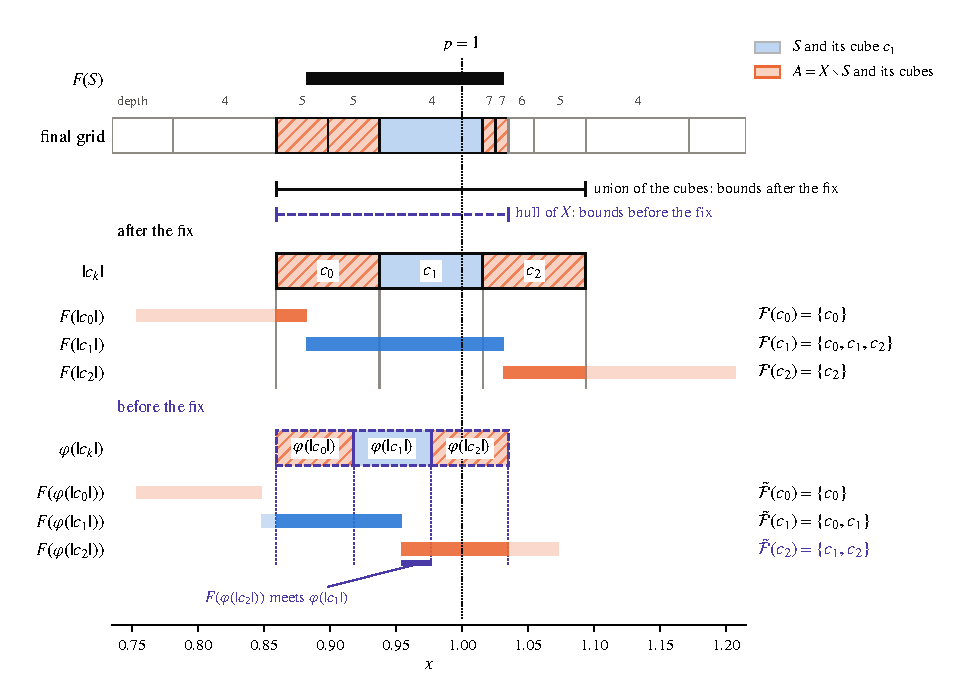
\includegraphics{bounds_e1_number_line.pdf}
\caption{E1 near the repeller $p=1$. Top: the cells of the final grid near the Morse set $S=[0.9375,1.015625]$ with their depths, and $F(S)$. $X=\cover F(S)$ consists of $S$ and the hatched cells of $A=X\setminus S$, two of which have depth $7$. Middle: the hull $[0.859375,1.03515625]$ of the cells of $X$, which bounded the complex before the fix, and the union $[0.859375,1.09375]$ of the cubes, which bounds it after the fix. After the fix: the boxes $|c_0|$, $|c_1|$, $|c_2|$ of the cubes of depth $4$, their images $F(|c_k|)$, and the cubes $\Fc(c_k)$ that each image meets under the rule of Section~\ref{sec:cubes}. Light parts of an image lie outside the bounds and are clamped. Before the fix: the boxes $\varphi(|c_k|)$ on which $F$ was evaluated, with $\varphi(x)=0.859375+0.75(x-0.859375)$, their images $F(\varphi(|c_k|))$ and the map $\Ft$. For $c_2\in A'$, the image $F(\varphi(|c_2|))$ meets $\varphi(|c_1|)$, so $c_1\in\Ft(c_2)$ and $\Ft(A')\cap X'\not\subseteq A'$. The boxes $\varphi(|c_k|)$ are those that $F$ received on 1.5.2, 1.3.3+fork.6 and 0e21503, and the boxes $|c_k|$ those it received on 96642f2.}\label{fig:e1line}
\end{figure}

\begin{figure}[tbp]
\centering
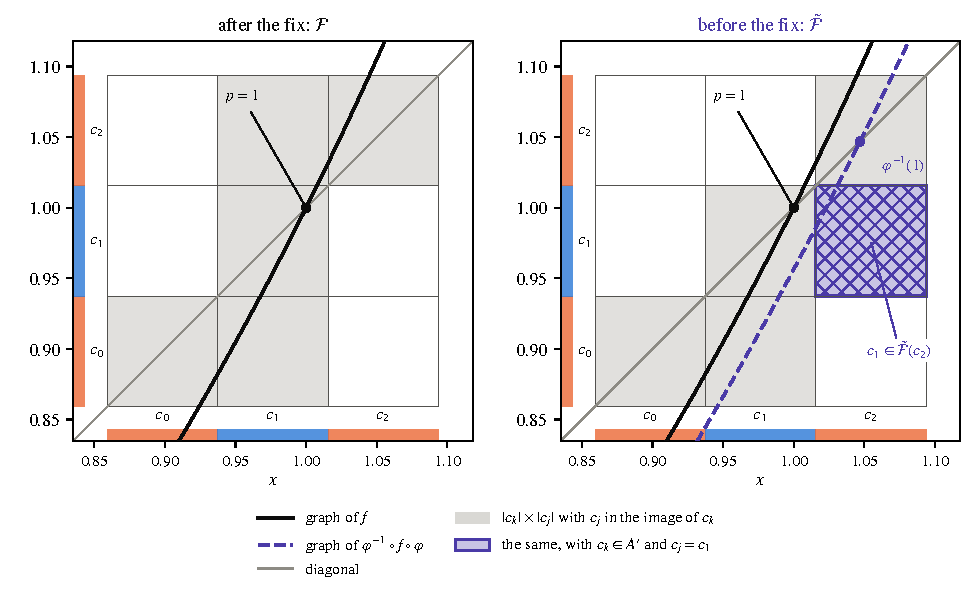
\includegraphics{bounds_e1_graph.pdf}
\caption{E1 on the cubes $c_0$, $c_1=S$ and $c_2$, with bands along the axes for $S$ (blue) and $A'$ (orange). The squares $|c_k|\times|c_j|$ with $c_j\in\Fc(c_k)$ after the fix (left) and $c_j\in\Ft(c_k)$ before it (right), with the graph of $f$ and the diagonal. By Proposition~\ref{prop:old}, $\Ft(c_k)$ consists of the cubes $c'$ whose half-open boxes $[c')$ meet the clamped image of $|c_k|$ under $\varphi^{-1}\circ f\circ\varphi$ (dashed), and the fixed point $\varphi^{-1}(1)=1.046875$ of this map lies in $|c_2|$. The hatched square $|c_2|\times|c_1|$ is the failure $c_1\in\Ft(c_2)$ of the condition $\Ft(A')\cap X'\subseteq A'$.}\label{fig:e1graph}
\end{figure}

\subsection{E2 and E3}\label{sec:e2e3}

In E2 the Morse set $S=[0.975,1.05]$ contains the repeller $1$. The cells of $A$ are $[0.9375,0.95625]$ and $[0.95625,0.975]$, of depth $6$, and $[1.05,1.0875]$ and $[1.0875,1.125]$, of depth $5$, so the cubes are $c_0=[0.9,0.975]$, $c_1=S$ and $c_2=[1.05,1.125]$, and the bounds before the fix were $[0.9375,1.125]$ instead of $[0.9,1.125]$. Then $\varphi(x)=0.9375+(5/6)(x-0.9)$ and $\varphi^{-1}(1)=0.975$, the common end of $c_0$ and $c_1$, so the fixed point $1$ lies on the old grid line $1.0$. The boxes $\varphi(|c_k|)$ were $[0.9375,1.0]$, $[1.0,1.0625]$ and $[1.0625,1.125]$, with the images $[0.882352941,1.0]$, $[1.0,1.133333333]$ and $[1.133333333,1.285714286]$. The first image ends on the grid line $1.0$, which the half-open box of $c_1$ contains, so $\Ft(c_0)=\{c_0,c_1\}$. The third image lies above the bound $1.125$, so $\Ft(c_2)=\emptyset$, and $\Ft(c_1)=\{c_1,c_2\}$. Over the vertex between $c_1$ and $c_2$, the closure of the images of the cubes that contain it is $|c_1|\cup|c_2|$, nothing is removed since $\Ft(c_2)=\emptyset$, and a single vertex is not a boundary there. So no vertex choice yields a preboundary. Accordingly 1.5.2 and 0e21503 annotate $S$ with $\undefidx$, \code{ComputeConleyMorseGraph} of 1.3.3+fork.6 raises \code{RuntimeError}, and \code{ComputeConleyIndex} returns $\undefidx$ for $\Ft$ on 1.5.2, 0e21503 and 96642f2 and raises \code{RuntimeError} on 1.3.3+fork.6 (computed). With closed boxes, $\Ft$ would map $c_0\mapsto\{c_0,c_1\}$, $c_1\mapsto\{c_0,c_1,c_2\}$ and $c_2\mapsto\{c_2\}$, the condition would still fail, and \code{ComputeConleyIndex} returns $(0,x-1)$ for this map. So the undefined result rests on the half-open boxes of \code{CubicalComplex::cover}. After the fix, $\Fc$ maps $c_0\mapsto\{c_0\}$, $c_1\mapsto\{c_0,c_1,c_2\}$ and $c_2\mapsto\{c_2\}$, and every build returns $(0,x-1)$ for $\Fc$.

In E3 the Morse set $S=[0.6625,0.709375]$ contains $p=0.6875$, the three cells of $A$ have depth $7$, and the cubes are $c_0=[0.615625,0.6625]$, $c_1=S$ and $c_2=[0.709375,0.75625]$. The bounds before the fix were $[0.656640625,0.72109375]$ instead of $[0.615625,0.75625]$, so the cubes had width $0.021484375$ instead of $0.046875$. Before the fix $\Ft$ mapped $c_0\mapsto\{c_1,c_2\}$, $c_1\mapsto\{c_0,c_1\}$ and $c_2\mapsto\{c_0\}$, and after it $\Fc$ maps $c_0\mapsto\{c_2\}$, $c_1\mapsto\{c_0,c_1,c_2\}$ and $c_2\mapsto\{c_0\}$. Here $\varphi(x)=0.656640625+(11/24)(x-0.615625)$ and $\varphi^{-1}(p)=0.682954545$ lies in $S$, so the failure is the condition $\Ft(A')\cap X'\subseteq A'$ alone, at $c_0\mapsto c_1$. The lift on the line yields $0$ for two of the three vertex choices and $-1$ for the third, the old builds returned $(0,0)$, and \code{ComputeConleyIndex} returns $(0,0)$ for $\Ft$ and $(0,x+1)$ for $\Fc$ on all four builds (computed).

\subsection{Dimension two}\label{sec:2d}

In E4 the Morse set of the saddle $(0,1)$ is $S=[0,0.078125]\times[0.9375,1.015625]$, of depth $8$ (Figure~\ref{fig:e4}), and
\[
F(S)=[0,0.040650407]\times[0.882352941,1.031746032].
\]
$X$ has $12$ cells, and the $11$ cells of $A$ are deeper than $S$: four cells of depth $10$ below $S$, and above it one cell of depth $11$, two of depth $13$ and four of depth $14$. The cubes are $c_k$ with offsets $(0,k)$, $k=0,1,2$. The cell of depth $11$, $[0.0390625,0.05859375]\times[1.015625,1.0546875]$, ends the hull of the cells of $X$ at $y=1.0546875$, below the upper end $1.09375$ of $c_2$, so the bounds were short along $y$, the unstable direction. Along $y$, $\varphi(y)=0.859375+(5/6)(y-0.859375)$, and the image of $\varphi(|c_2|)$ meets the half-open box $\varphi([c_1))$:
\[
\begin{aligned}
F(\varphi(|c_2|))&=[0,0.040650407]\times[0.979381443,1.115702479],\\
\varphi([c_1))&=[0,0.078125)\times[0.924479167,0.989583333).
\end{aligned}
\]
So $\Ft$ maps $c_0\mapsto\{c_0\}$, $c_1\mapsto\{c_0,c_1\}$ and $c_2\mapsto\{c_1,c_2\}$, and $\Fc$ maps $c_0\mapsto\{c_0\}$, $c_1\mapsto\{c_0,c_1,c_2\}$ and $c_2\mapsto\{c_2\}$. Along $y$, $\varphi^{-1}(1)=1.028125$ lies in $c_2$. \code{ComputeConleyIndex} returns $(0,0,0)$ for $\Ft$ and $(0,x-1,0)$ for $\Fc$ (computed).

\begin{figure}[tbp]
\centering
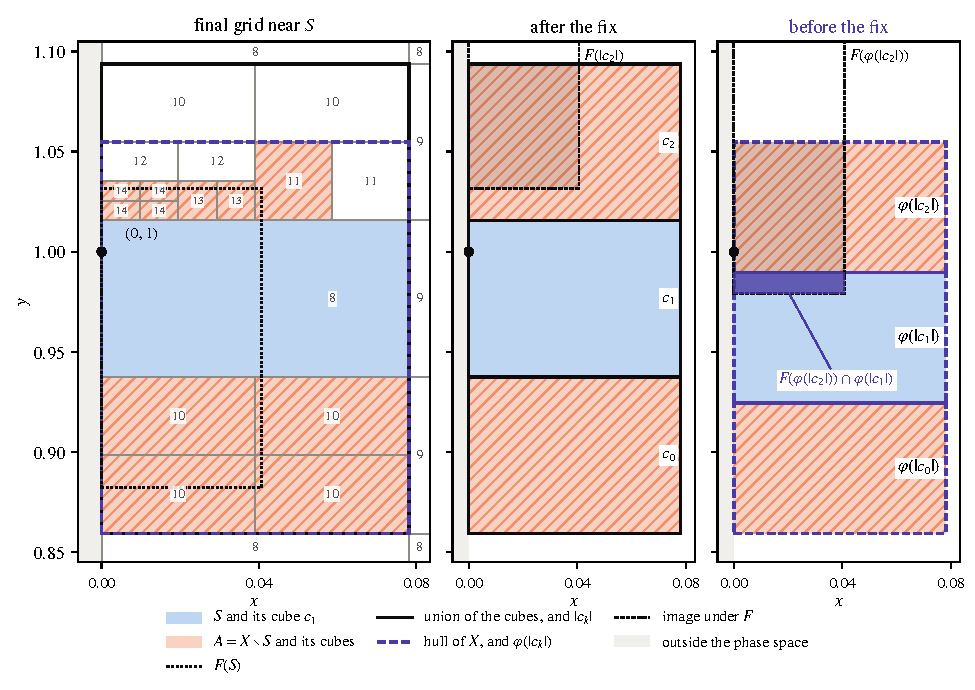
\includegraphics{bounds_e4_saddle.pdf}
\caption{E4 near the saddle $(0,1)$. Left: the cells of the final grid near the Morse set $S=[0,0.078125]\times[0.9375,1.015625]$ of depth $8$, with their depths, $F(S)$ (dotted), the hatched cells of $A=X\setminus S$ (depths $10$ to $14$), the union of the boxes $|c_k|$ of the cubes $c_k$ with offsets $(0,k)$ (solid), and the hull of the cells of $X$ (dashed), which ends at $y=1.0546875$ instead of $1.09375$. Middle: the boxes $|c_k|$ after the fix and the image $F(|c_2|)$, which meets only $|c_2|$. Right: the boxes $\varphi(|c_k|)$ on which $F$ was evaluated before the fix, with $\varphi(y)=0.859375+(5/6)(y-0.859375)$ along $y$. The image $F(\varphi(|c_2|))$ meets $\varphi(|c_1|)$ (filled), so $c_1\in\Ft(c_2)$. The gray strip $x<0$ lies outside the phase space.}\label{fig:e4}
\end{figure}

For the saddle $(1,0)$ of E4, the bounds are short along $x$ with the numbers of E1, and $\Ft$ is the transpose of the map of $(0,1)$. \code{ComputeConleyIndex} returns $(0,x-1,0)$ for this $\Ft$, the correct value, and so do the old builds, although the same structure in the other orientation yields $(0,0,0)$ at $(0,1)$. So the old output depends on how chomp orders the cubes. The two outputs are computed, and this cause is inferred. For the repeller $(1,1)$, $X$ has $30$ cells, $29$ of them deeper than $S$, the bounds are short along $x$, and $\Ft$ maps the cube $(2,1)$ of $A'$ into $S'=\{(1,1)\}$. \code{ComputeConleyIndex} returns $(0,0,0)$ for $\Ft$ and $(0,0,x-1)$ for $\Fc$.

\begin{remark}\label{rem:lift2d}
In dimension two, a preboundary is determined only up to boundaries of $2$-chains in its fiber, so the lift of $\Ft$ is not determined by the vertex choice. For the repeller $(1,1)$ of E4 under $\Ft$, every element of $\F$ is attained as the coefficient of the lift of the generator, for each of the $12$ vertex choices, by some preboundary over an edge of $S$, and the $0$ of chomp is one of these values. For the saddles, a representative of the generator by a single edge yields $0$ for $4$ of the $6$ vertex choices and the generator for the other $2$. These results come from an earlier analysis whose scripts are not part of this report.
\end{remark}

In E5, the Morse sets of $(0,1)$, $(1,0)$ and $(1,1)$ have bounds short along an expanding axis, $[0.9375,1.125]$ instead of $[0.9,1.125]$. In each of them a cube of $A'$ maps into $S'$, and some cubes of $A'$ have empty images: $(0,2)$ for $(0,1)$, $(2,0)$ for $(1,0)$, and $(2,0)$, $(2,1)$ and $(2,2)$ for $(1,1)$. As in E2, the index is undefined on 1.5.2 and 0e21503, and 1.3.3+fork.6 raises \code{RuntimeError}. The Morse set of $(0,1)$ is the two-dimensional form of E2.

E6 is the control. Its bounds are short for $(0,1)$, $(1,0)$ and $(1,1)$, for example $[0.75,1.125]$ instead of $[0.75,1.2]$ along $y$ for $(0,1)$, and $15$ of the $20$ evaluations of $F$ in the computation of the Conley indices are off the bisection tree on 1.5.2 and 0e21503, $55$ of $60$ on 1.3.3+fork.6, and none on master. Nevertheless $\Ft=\Fc$ for all four Morse sets, and every build returns the annotation of the linearization. This rests on exact contacts with the old grid lines $0.75$, $0.875$, $1.0$ and $1.125$ along $y$. For $(0,1)$, the image of $\varphi(|c_2|)$ has $y$-part $[1.0,1.285714286]$, whose lower end $f(1)=1$ lies on the line between the $y$-parts $[0.875,1.0]$ and $[1.0,1.125]$ of $\varphi(|c_1|)$ and $\varphi(|c_2|)$, and \code{CubicalComplex::cover} assigns only $c_2$. The fixed point $\varphi^{-1}(1)=1.05$ is the common end of $c_1=[0.9,1.05]$ and $c_2=[1.05,1.2]$. With closed boxes, $\Ft$ would also map $c_2$ into $c_1$, the condition would fail, and \code{ComputeConleyIndex} returns $(0,0,0)$ for this map at $(0,1)$. For $(1,0)$ and $(1,1)$ closed boxes break the condition as well, although \code{ComputeConleyIndex} still returns $(0,x-1,0)$ and $(0,0,x-1)$ (computed). So the correct annotations of E6 do not show that the old boxes are harmless.

\subsection{Where the deeper cells come from}\label{sec:scope}

By Corollary~\ref{cor:scope}, the defect needs $\dmax>\dmin$ and a cell of $X$ deeper than $S$ whose ancestor sticks out of the hull of the cells of $X$. In E1 the uniform run of depth $4$ has five Morse sets: $[0,0.078125]$ with $(x-1,0)$, $[0.078125,0.15625]$ with $(0,0)$, $c_0=[0.859375,0.9375]$ and $c_2=[1.015625,1.09375]$ with $(0,0)$, and $S$ with $(0,x-1)$. So $c_0$ and $c_2$ are cells with a self-loop and trivial index at depth $4$. In the adaptive run, the regions of $c_0$ and $c_2$ hold cells of depths $5$, $5$ and $7$, $7$, $6$, $5$ and no Morse set. With Section~\ref{sec:hierarchy}, this indicates that the hierarchy refined $c_0$ and $c_2$, discarded them, and joined their refinements into the final grid. The hierarchy was not instrumented to confirm this. E2 and E3 have the same structure: the uniform run of depth $4$ of E2 has the Morse sets $[0.9,0.975]$ and $[1.05,1.125]$ with $(0,0)$, and that of E3 has the Morse set $\{c_0,c_2\}$ with $(0,0)$ next to $S$.

\begin{remark}\label{rem:sweep}
An earlier sweep of $729$ adaptive runs with $\dmin<\dmax$, for $x\mapsto-2x/(1+3x^2)$ on $60$ domains and the logistic map with $r\in\{3.2,3.3,3.4\}$ on $7$ domains, under $9$ models each, found the annotation $(0,x+1)$ for the fixed point on master in $670$ runs. The merge 0e21503 differs in $134$ of them, with $97$ trivial and $37$ undefined annotations. In the other $59$ runs the fixed point is not isolated from the attracting $2$-cycle, and both builds return $(x-1,0)$. In the models tested, $\dinit$ did not change the outcome. The scripts of that sweep are not part of this report.
\end{remark}

\subsection{The fix and the tests}\label{sec:fix}

Commit 577d988 uses the geometry of the ancestor of depth $d$ for a cell deeper than $d$ in the computation of the bounds (Listing~\ref{lst:new}). The bounds are then $[a_i,b_i]$, and the code evaluates $F$ on the cubes, which are boxes of the bisection tree. Three computed facts attribute the change of the annotations to this commit, although master contains other changes. First, \code{ComputeConleyIndex}, which receives the map on cubes and no geometry, returns for $\Fc$ the annotation of master, for all $18$ Morse sets and on each of the four builds. For $\Ft$ it returns the annotation of each old build wherever that build returns one, and on 1.3.3+fork.6 it raises \code{RuntimeError} for the sets of E2 and E5 whose index is undefined on 1.5.2 and 0e21503. On master it returns the old annotations when given $\Ft$, so the change lies in the map on cubes and not in the lift. Second, on master no cube is evaluated more than once, since for every Morse set the evaluations on cubes are as many as the distinct boxes, so the retry at \path{chomp/ConleyIndex.h}:190--193, which would evaluate cubes again, did not run. Third, for all $70$ Morse sets that the runs reach on the four builds, the boxes that $F$ receives in the computation of the Conley indices are the cells of $S$ and the boxes that Proposition~\ref{prop:old} predicts, with deviation $0$: $\varphi(|c|)$ on the old builds and $|c|$ on master.

The tests in \path{tests/test_conley_geometry_regressions.py}, added with the fix, check the annotations of the fixed points of E1, E2, E4 and E5, and that every box that $F$ receives in \code{ComputeConleyMorseGraph} is a box of the bisection tree, on E1, E2, E4, E5 and E6. They also run E6 through \code{PrecomputedBoxMap}, which rejects boxes off the lattice of the bisection tree. All $11$ tests pass on 96642f2 and fail on 0e21503 (computed).

The fixed code does not check that $(X',A')$ is a combinatorial index pair for $\Fc$. A cube that replaces a deeper cell of $A$ can contain cells outside $X$, and nothing in the construction keeps such a cube from mapping into $S'$. The condition holds for all $18$ Morse sets here.

\section{Part II: the hierarchy with box maps that are not monotone}\label{sec:leslie}

\subsection{The Leslie map}\label{sec:dynamics}

Let $\alpha=19.6$, $\beta=23.68$ and
\[
f(x,y)=\left((\alpha x+\beta y)e^{-0.1(x+y)},\ 0.7x\right)=(f_1,f_2)
\]
on $Q=[-0.001,90]\times[-0.001,70]$, with the model of \code{leslie\_model} in \path{tests/test_map_graph_cache.py}, $\mathrm{Model}(\dmin,\dmax,Q,F)$. The cells of depth $1$ and $2$ that matter are
\[
\begin{aligned}
L&=[-0.001,44.9995]\times[-0.001,70], & C&=[44.9995,90]\times[-0.001,70],\\
L_b&=[-0.001,44.9995]\times[-0.001,34.9995], & C'&=[-0.001,44.9995]\times[34.9995,70].
\end{aligned}
\]
Since $f_2=0.7x$, the hull of $f(B)$ for a box $B$ follows from the extremes of $f_1$ on $B$.

\begin{lemma}\label{lem:hull}
Let $\ell=\alpha x+\beta y$. Then $\partial f_1/\partial x=(\alpha-0.1\ell)e^{-0.1(x+y)}$ and $\partial f_1/\partial y=(\beta-0.1\ell)e^{-0.1(x+y)}$, and $f_1$ has no critical point. On a box, the minimum of $f_1$ is attained at a corner, and its maximum at a corner or at one of the points $(10-(\beta/\alpha)c,\,c)$ of an edge $y=c$ and $(c,\,10-(\alpha/\beta)c)$ of an edge $x=c$ that lie on the box, where $f_1$ takes the values $10\alpha\,e^{-1-0.1(1-\beta/\alpha)c}$ and $10\beta\,e^{-1-0.1(1-\alpha/\beta)c}$. On $C$, $f_1$ decreases in both variables.
\end{lemma}

\begin{proof}
A critical point would need $\alpha=0.1\ell=\beta$. On an edge $y=c$, $\partial f_1/\partial x$ vanishes only where $\ell=10\alpha$, that is, at $x=10-(\beta/\alpha)c$, and it changes sign from $+$ to $-$ there, since $\ell$ increases with $x$. So the extremes of $f_1$ on the boundary of a box lie at the corners and at these points, which are maxima along their edges, and the edges $x=c$ are similar. On $C$, $\ell\geq44.9995\alpha-0.001\beta=881.967>10\beta>10\alpha$, so both partial derivatives are negative.
\end{proof}

Three box maps are compared. $\Phi(B)$ is the hull of the values of $f$ at the four corners of $B$, \code{CMGDB.BoxMap(f, B)}. $\Phipad(B)$ is $\Phi(B)$ widened on each side by the widths of $B$, \code{CMGDB.BoxMap(f, B, padding=True)}. $\Phihull(B)$ is $\hull f(B)$, computed from Lemma~\ref{lem:hull}, widened by $10^{-9}(1+m)$ in the first coordinate, where $m$ is the largest absolute value of an end of the first coordinate, and by $10^{-12}$ in the second.

\begin{proposition}\label{prop:fixed}
The fixed points of $f$ in $\R^2$ are $0$ and $p^*=(x^*,0.7x^*)$ with $x^*=\ln(36.176)/0.17=21.108211$. The eigenvalues of $Df(0)$ are $\lambda_u=(19.6+\sqrt{450.464})/2=20.412069$ and $\lambda_s=-0.812069$, with the eigenvectors $(1,0.034293)$ and $(1,-0.861996)$. The eigenvalues of $Df(p^*)$ are $-0.784513\pm0.635539i$, of modulus $1.009639$. So $0$ is a hyperbolic saddle with a positive unstable eigenvalue, and $p^*$ is a repelling focus with $\det Df(p^*)=1.019370>0$.
\end{proposition}

\begin{proof}
$f(z)=z$ if and only if $y=0.7x$ and $x=(\alpha+0.7\beta)\,x\,e^{-0.17x}$, with $\alpha+0.7\beta=36.176$. The eigenvalues $\lambda$ of $Df(0)$ solve $\lambda^2-\alpha\lambda-0.7\beta=0$, with eigenvectors $(\lambda,0.7)$. At $p^*$, $e^{-0.17x^*}=1/36.176$ and $\alpha x^*+\beta y^*=36.176\,x^*$, so
\[
Df(p^*)=\begin{pmatrix}\alpha/36.176-0.1x^*&\beta/36.176-0.1x^*\\0.7&0\end{pmatrix}=\begin{pmatrix}-1.569025&-1.456244\\0.7&0\end{pmatrix},
\]
with trace $-1.569025$ and determinant $1.019370$.
\end{proof}

The rest of the dynamics is numerical (\path{leslie_dynamics.py}). Newton's method for $f^n(z)=z$, $n=1,\dots,12$, from a $91\times71$ grid of seeds finds four orbits with all points in $Q$: $0$, $p^*$, an attracting $3$-cycle $a_3$ and a saddle $3$-cycle $s_3$,
\[
\begin{aligned}
a_3&:\ (7.524656,0.499081)\mapsto(71.409072,5.267260)\mapsto(0.712973,49.986350),\\
s_3&:\ (19.212912,1.304927)\mapsto(52.362602,13.449038)\mapsto(1.864181,36.653822).
\end{aligned}
\]
The eigenvalues of $Df^3$ are $0.053550$ and $-0.808958$ along $a_3$, and $2.384270$ and $0.068732$ along $s_3$. This is evidence, not a proof, that there are no other periodic orbits of these periods. For both cycles, the second point lies in $C$ and the third in $C'$. The orbit of $(30,20)$ after $100000$ steps fills a closed curve $\Gamma$ in $[12.2812,30.7980]\times[8.5968,21.5586]$, star-shaped about $p^*$, on which the angle about $p^*$ advances by $1.47268$ to $2.98822$ per step, with rotation number $0.387850$ and no period up to $2000$. The Lyapunov exponents along it are $-5.14\times10^{-6}$ and $-0.01958$. We infer that $\Gamma$ is an attracting invariant circle, on which $f$ has degree $1$ since a lift $\theta\mapsto\theta+\delta(\theta)$ with $0<\delta<2\pi$ has degree $1$, and let $K$ be the closed disk bounded by $\Gamma$. Of the $101441$ seeds of a $361\times281$ grid of $[0,90]\times[0,70]$, $63926$ converge to $a_3$ and $37514$ to $\Gamma$ within $5000$ steps, and the remaining seed is the origin. At each point of $s_3$, one branch of $W^u(s_3)$ goes to $\Gamma$ and the other to $a_3$ (Figure~\ref{fig:phase}). Table~\ref{tab:expected} lists the indices that this structure implies.

\begin{figure}[tbp]
\centering
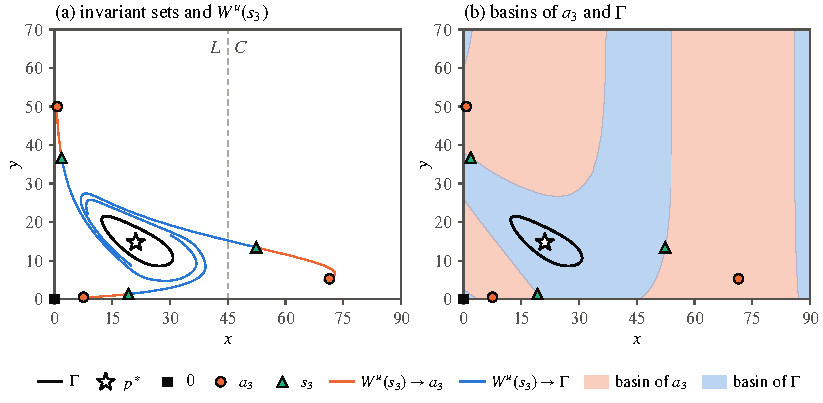
\includegraphics[width=\textwidth]{leslie_phase_portrait.pdf}
\caption{The Leslie map on $Q$ (computed). (a) The fixed points $0$ (square) and $p^*$ (star), the invariant circle $\Gamma$ (the orbit of $(30,20)$ after $100000$ steps), the attracting $3$-cycle $a_3$ (circles) and the saddle $3$-cycle $s_3$ (triangles). At each point of $s_3$, one branch of $W^u(s_3)$ goes to $a_3$ (orange) and the other to $\Gamma$ (blue), drawn as $18$ images under $f^3$ of a fundamental domain. The dashed line $x=44.9995$ separates the cells $L$ and $C$ of depth $1$, and each $3$-cycle has a point in $C$. (b) The seeds of a $361\times281$ grid that converge to $a_3$ (orange, $63926$ seeds) and to $\Gamma$ (blue, $37514$ seeds) within $5000$ steps.}\label{fig:phase}
\end{figure}

\begin{table}[tbp]
\centering
\caption{Conley indices of the invariant sets of the Leslie map, shown as annotations. Each index follows from the property in the third column, and the last column says what that property rests on. $J$ is the union of $s_3$, the three branches of $W^u(s_3)$ that go to $\Gamma$, and $K$.}\label{tab:expected}
\small
\begin{tabular}{llll}
\toprule
set & annotation & property & rests on \\
\midrule
$\{0\}$ & $(0,x-1,0)$ & saddle, $\lambda_u>0$ & Proposition~\ref{prop:fixed} \\
$\{p^*\}$ & $(0,0,x-1)$ & repeller, $\det Df(p^*)>0$ & Proposition~\ref{prop:fixed} \\
$a_3$ & $(x^3-1,0,0)$ & attracting $3$-cycle & the computed cycle \\
$s_3$ & $(0,x^3-1,0)$ & saddle $3$-cycle, unstable eigenvalue of $Df^3$ positive & the computed cycle \\
$\Gamma$ & $(x-1,x-1,0)$ & attracting circle, $f|_\Gamma$ of degree $1$ & the inferred circle \\
$K$ & $(x-1,0,0)$ & attractor, a disk & the inferred circle \\
$J$ & $(0,x^2+x+1,0)$ & Proposition~\ref{prop:J} & the inferred structure \\
\bottomrule
\end{tabular}
\end{table}

For $s_3$, the index map on $H_1=\F^3$ is a cyclic permutation times signs whose product is the sign of the unstable eigenvalue of $Df^3$, which is positive, and a diagonal change of signs makes it the cyclic permutation $P$. The index of $J$ needs an argument, since a connecting orbit alone does not make a connecting homomorphism nonzero.

\begin{lemma}\label{lem:H0}
Let $J$ be a connected isolated invariant set of $f$, and suppose that $J$ has a neighborhood $V$ such that every neighborhood of $J$ contains a point whose forward orbit leaves $V$. Then the index map is nilpotent on $H_0$, and the annotation of $J$ has $0$ in degree $0$.
\end{lemma}

\begin{proof}
Let $(P_1,P_0)$ be an index pair for $J$ with $P_1\subseteq V$ that is homeomorphic to a finite simplicial pair, for example a pair of cubical sets. Such pairs exist since $J$ is isolated~\cite{FR00,Mro99}, and the filtration pairs of~\cite{FR00} satisfy (i) to (iii) of Definition~\ref{def:pair}. Then $P_1$ has finitely many components, each path connected and open in $P_1$, and the components that do not meet $P_0$ form a basis of $H_0(P_1,P_0;\F)$. For such a component $Z$, $f(Z)\subseteq P_1$ by (iii) of Definition~\ref{def:pair}, and $f(Z)$ is connected, so it lies in one component $\sigma(Z)$ of $P_1$. The index map takes $[Z]$ to $[\sigma(Z)]$ if $\sigma(Z)\cap P_0=\emptyset$ and to $0$ otherwise. Suppose that it is not nilpotent on $H_0$. Then there are components $Z_1,\dots,Z_m$ that do not meet $P_0$ with $\sigma(Z_k)=Z_{k+1}$ and $\sigma(Z_m)=Z_1$, and their union $U$ satisfies $f(U)\subseteq U$. So $\bigcap_{n\geq0}f^n(U)$ is a nonempty compact invariant subset of $P_1\setminus P_0$, which lies in $J$, and $U$ contains the component $Z_J$ of $P_1$ that contains the connected set $J$. Since $P_1$ is a neighborhood of $J$ and $Z_J$ is open in $P_1$, $Z_J$ is a neighborhood of $J$, and the forward orbit of every point of $Z_J$ stays in $U\subseteq V$, which contradicts the hypothesis.
\end{proof}

\begin{proposition}\label{prop:J}
Suppose that $K$ is an attractor whose index has the annotation $(x-1,0,0)$, that the index of $s_3$ is $\F^3$ in degree $1$ with the index map $P$, and that $J$ is an isolated invariant set in which $(K,s_3)$ is an attractor-repeller pair. Suppose further that $J$ is connected and that the other three branches of $W^u(s_3)$ go to $a_3\notin J$. Then the Conley index of $J$ is $0$ in degrees $0$ and $2$ and $\F^2$ in degree $1$, with an index map of characteristic polynomial $x^2+x+1$, so its annotation is $(0,x^2+x+1,0)$.
\end{proposition}

\begin{proof}
Let $N_0\subseteq N_1\subseteq N_2$ be an index triple of the attractor-repeller pair, that is, $(N_2,N_0)$, $(N_1,N_0)$ and $(N_2,N_1)$ are index pairs for $J$, $K$ and $s_3$. Such triples exist~\cite{FR00}, and we take one homeomorphic to a finite simplicial triple, as for the pair in the proof of Lemma~\ref{lem:H0}, so that its homology is finite-dimensional. Since $f(N_1)\subseteq N_1\cup f(N_0)$ by (iii) of Definition~\ref{def:pair}, the three index maps are induced by $f$ as a map of triples into $(N_2\cup f(N_0),N_1\cup f(N_0),N_0\cup f(N_0))$, so they commute with the maps of the long exact sequence of the triple. Restriction to invertible parts is exact on finite-dimensional vector spaces with an endomorphism, since it is the image of the idempotent of the Fitting decomposition, a polynomial in the endomorphism. Denote by $\CH_k$ the invertible part of the index map in degree $k$. With $\CH_*(K)=(\F,0,0)$ and $\CH_*(s_3)=(0,\F^3,0)$, the sequence yields $\CH_2(J)=0$ and the exact sequence
\[
0\to\CH_1(J)\to\F^3\xrightarrow{\ \partial\ }\F\to\CH_0(J)\to0,
\]
with $\partial\circ P=\partial$. Let $V$ be a neighborhood of $J$ whose closure does not contain $a_3$. Every neighborhood of $J$ contains points of the branches that go to $a_3$, whose forward orbits leave $V$, so Lemma~\ref{lem:H0} applies, and $\CH_0(J)=0$. Hence $\partial$ is onto, and since $P$ permutes the basis vectors $e_1,e_2,e_3$ cyclically, $\partial(e_1)=\partial(e_2)=\partial(e_3)\neq0$. So $\CH_1(J)$ is isomorphic to $\{v\in\F^3:v_1+v_2+v_3=0\}$, on which $P$ has the characteristic polynomial $(x^3-1)/(x-1)=x^2+x+1$. This polynomial is irreducible over $\F$, since its discriminant $-3\equiv2$ is not a square modulo $5$, so it is the only invariant factor.
\end{proof}

The computed annotations agree with Proposition~\ref{prop:J}: the Morse set of the uniform run of depth $14$ with $\Phi$ that contains $p^*$, $\Gamma$ and $s_3$, with $2023$ cells, and that of the run $16/18$ with $\Phipad$, with $8636$ cells, are both annotated $(0,x^2+x+1,0)$.

\subsection{Morse decompositions}\label{sec:morse}

Table~\ref{tab:morse} lists the Morse sets of ten runs, and Figure~\ref{fig:morse16} shows four of them. A Morse set is identified by the invariant sets that it contains: $0$, $p^*$, the points of $a_3$ and $s_3$, and $2000$ points of $\Gamma$. In every run the set that contains $p^*$ contains all points of $\Gamma$, so no run separates $p^*$ from $\Gamma$. The eigenvalues of $Df(p^*)$ have modulus $1.0096$, so the repulsion at $p^*$ is weak. In the runs $12/14$ and $16/18$ with $\Phi$, no Morse set contains a point of $a_3$ or $s_3$. In the order of the display in Section~\ref{sec:dynamics}, the second points of $a_3$ and $s_3$ lie in $C$, the third points lie in $C'$, and the first points lie in cells of depths $7$ and $10$ that are in no Morse set. The uniform runs of depths $16$ and $18$ with $\Phi$ and the run $16/18$ with $\Phihull$ find $a_3$, $s_3$ and the set around $p^*$ and $\Gamma$ with the indices of Table~\ref{tab:expected}, the last one on a grid of $8759$ cells instead of $65536$. The Morse set that contains $0$ is annotated $(0,0,0)$ in every run, for reasons unrelated to the hierarchy (Section~\ref{sec:origin}). The Morse sets of $3$ to $13$ cells that contain none of these invariant sets were not analyzed.

\begin{table}[tbp]
\centering
\caption{Morse sets of the Leslie map (computed, \path{outputs/leslie_morse_cmgdb-1.5.3_fork.7.dev0-96642f2.txt}, the same on all four builds). For each run, the number of cells of the final grid, and for each Morse set the invariant sets that it contains, its number of cells and its annotation. The uniform runs use $\Phi$.}\label{tab:morse}
\small
\begin{tabular}{llrl}
\toprule
run (cells) & contents & cells & annotation \\
\midrule
$\Phi$, $12/14$ ($636$) & $p^*$, $\Gamma$ & $525$ & $(0,x+1,0)$ \\
 & $0$ & $1$ & $(0,0,0)$ \\
$\Phi$, $16/18$ ($7059$) & $p^*$, $\Gamma$ & $5570$ & $(x-1,0,0)$ \\
 & $0$ & $1$ & $(0,0,0)$ \\
uniform $12$ ($4096$) & $p^*$, $\Gamma$, $a_3$, $s_3$ & $809$ & $(x-1,0,0)$ \\
 & $0$ & $1$ & $(0,0,0)$ \\
uniform $14$ ($16384$) & $a_3$ & $73$ & $(x^3-1,0,0)$ \\
 & $p^*$, $\Gamma$, $s_3$ & $2023$ & $(0,x^2+x+1,0)$ \\
 & none, $3$ sets & $4$, $4$, $10$ & $(0,0,0)$ \\
 & $0$ & $1$ & $(0,0,0)$ \\
uniform $16$ ($65536$) & $a_3$ & $158$ & $(x^3-1,0,0)$ \\
 & $p^*$, $\Gamma$ & $5570$ & $(x-1,0,0)$ \\
 & $s_3$ & $89$ & $(0,x^3-1,0)$ \\
 & none, $4$ sets & $3$, $4$, $4$, $3$ & $(0,0,0)$ \\
 & $0$ & $1$ & $(0,0,0)$ \\
uniform $18$ ($262144$) & $a_3$ & $225$ & $(x^3-1,0,0)$ \\
 & $p^*$, $\Gamma$ & $15407$ & $(x-1,0,0)$ \\
 & $s_3$ & $73$ & $(0,x^3-1,0)$ \\
 & none, $3$ sets & $13$, $3$, $4$ & $(0,0,0)$ \\
 & $0$ & $1$ & $(0,0,0)$ \\
$\Phihull$, $12/14$ ($1073$) & $p^*$, $\Gamma$, $a_3$, $s_3$ & $810$ & $(x-1,0,0)$ \\
 & $0$ & $1$ & $(0,0,0)$ \\
$\Phihull$, $16/18$ ($8759$) & $a_3$ & $158$ & $(x^3-1,0,0)$ \\
 & $p^*$, $\Gamma$ & $5570$ & $(x-1,0,0)$ \\
 & $s_3$ & $89$ & $(0,x^3-1,0)$ \\
 & $0$ & $1$ & $(0,0,0)$ \\
$\Phipad$, $12/14$ ($1473$) & $p^*$, $\Gamma$, $a_3$, $s_3$ & $1128$ & $(x-1,0,0)$ \\
 & $0$ & $1$ & $(0,0,0)$ \\
$\Phipad$, $16/18$ ($14151$) & $a_3$ & $851$ & $(x^3-1,0,0)$ \\
 & $p^*$, $\Gamma$, $s_3$ & $8636$ & $(0,x^2+x+1,0)$ \\
 & $0$ & $1$ & $(0,0,0)$ \\
\bottomrule
\end{tabular}
\end{table}

\begin{figure}[tbp]
\centering
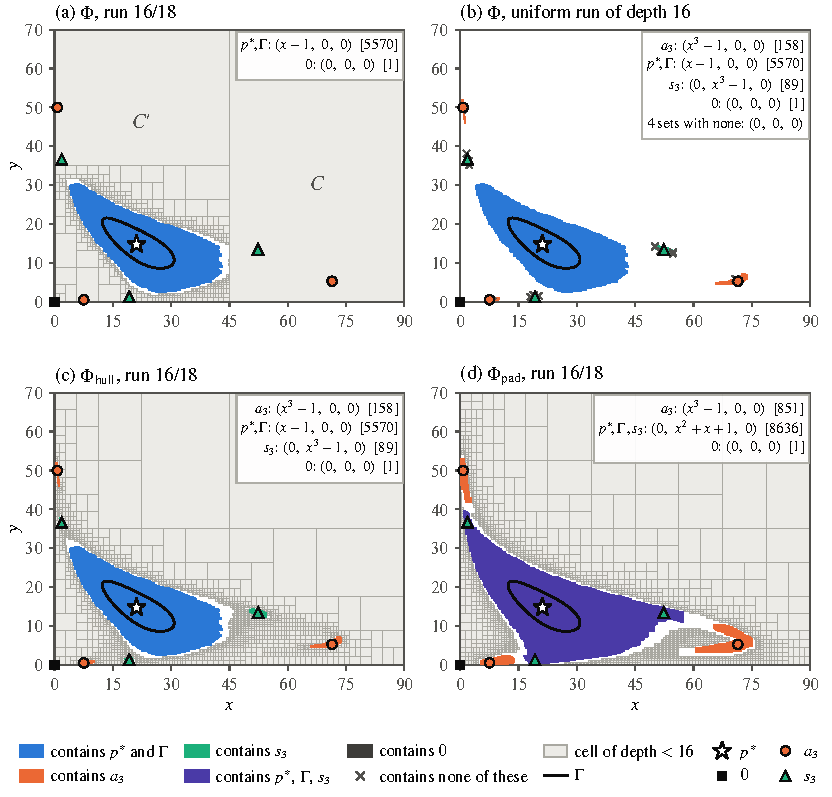
\includegraphics{leslie_morse_sets_16.pdf}
\caption{Morse sets at depth $16$ (computed): (a) the run $16/18$ with $\Phi$, (b) the uniform run of depth $16$ with $\Phi$, (c) the run $16/18$ with $\Phihull$, and (d) the run $16/18$ with $\Phipad$. Colors indicate the invariant sets that a Morse set contains, crosses mark the Morse sets that contain none of them, and the pale cells have depth less than $16$, the cells that the decomposition does not refine. Each panel lists the annotations, with the number of cells in brackets. In (a) the cells $C$ and $C'$ of depths $1$ and $2$ are never refined, and $a_3$ and $s_3$ lie in no Morse set. (b) and (c) find $a_3$, $s_3$ and $K$ with the indices of Table~\ref{tab:expected}, (c) on a grid of $8759$ cells instead of $65536$. In (d) $s_3$ and $K$ lie in one Morse set, annotated $(0,x^2+x+1,0)$, the annotation of the index of $J$.}\label{fig:morse16}
\end{figure}

The Morse graph of the run $16/18$ with $\Phihull$ is $0\to s_3\to\{p^*,\Gamma\}\to a_3$. Its edge $\{p^*,\Gamma\}\to a_3$ is not realized by a path of cells, since $\cover\Phihull(S)=S$ for the Morse set $S$ that contains $p^*$. It comes from the coarser grids, from which a hierarchical run inherits its edges. The paths of cells yield $0\to s_3$, $0\to\{p^*,\Gamma\}$, $0\to a_3$, $s_3\to\{p^*,\Gamma\}$ and $s_3\to a_3$, the order that the simulations suggest.

\subsection{The cell \texorpdfstring{$C$}{C}}\label{sec:cellC}

The four corners of $L$ have the images $(-0.0433,-0.0007)$, $(1.5117,-0.0007)$, $(9.7992,31.4996)$ and $(0.0257,31.4996)$. So $\Phi(L)=[-0.0433,9.7992]\times[-0.0007,31.4996]$, which meets $L$, and $\Phi(Q)=[-0.0433,1.5117]\times[-0.0007,63.0]$ meets $Q$ (computed, Figure~\ref{fig:levelone}). By Lemma~\ref{lem:hull}, the maximum of $f_1$ on $L$ is $87.1154$, attained at $(-0.001,10.000828)$, and $f(10,0)=(72.1044,7.0)$ lies in $C$. Also by Lemma~\ref{lem:hull}, $\Phi(C)=\hull f(C)=[0.0004,9.7992]\times[31.4996,63.0]$, which lies in $L$. Both $\Phi(L)$ and $\Phi(C)$ lie in $x\leq9.7992$, at distance more than $35$ from $C$, and \code{TreeGrid::cover} enlarges the cells along $x$ by $2^{-50}\cdot90.001<10^{-13}$ (Section~\ref{sec:hierarchy}). So on the grid $\{L,C\}$, $\cover\Phi(L)=\cover\Phi(C)=\{L\}$, for the cover of Section~\ref{sec:hierarchy} and for \code{TreeGrid::cover}.

\begin{proposition}\label{prop:depthone}
Suppose that $\Phi(Q)$ meets $Q$ and that $\cover\Phi(L)=\cover\Phi(C)=\{L\}$ on the grid $\{L,C\}$. Then every run with $\Phi$, $\dinit=0$ and $\dmin\geq1$ has the same node of depth $1$, whose graph has the edges $L\to L$ and $C\to L$ and whose only Morse set is $\{L\}$, and $C$ is a cell of the final grid of every such run.
\end{proposition}

\begin{proof}
The root has the grid $\{Q\}$ and, since $\Phi(Q)$ meets $Q$, the Morse set $\{Q\}$. Its child has the grid $\{L,C\}$, and by hypothesis the graph of this grid has the edges $L\to L$ and $C\to L$ and no other. So $\{L\}$ is the only strongly connected component with a cycle, and no node refines $C$. The grid of the node of depth $1$ enters the final grid, possibly through the grid of a discarded node, and in both cases $C$ is one of its cells.
\end{proof}

At depth $2$, $L$ splits into $L_b$ and $C'$. The boxes $\Phi(L_b)=[-0.0433,25.0304]\times[-0.0007,31.4996]$ and $\Phi(C')=[0.0257,25.0304]\times[-0.0007,31.4996]$ meet $Q$ only in $L_b$ and lie in $y\leq31.4996$, at distance more than $3.4$ from $C'$, so on the grid $\{L_b,C'\}$ the cover of each is $\{L_b\}$, and $C'$ is not refined either (computed). Since $f_2=0.7x\leq0.7\cdot44.9995=31.49965$ on $L$, $f(L)$ does not meet $C'$, and only $C$ maps into $C'$. The edge $C\to C'$ is not seen at depth $2$, because $C$ is not in the grid of that node. Every orbit of $a_3$ and $s_3$ passes through $C$ and $C'$, and in both adaptive runs with $\Phi$ the cells that contain the first points of $a_3$ and $s_3$ have depths $7$ and $10$.

\begin{figure}[tbp]
\centering
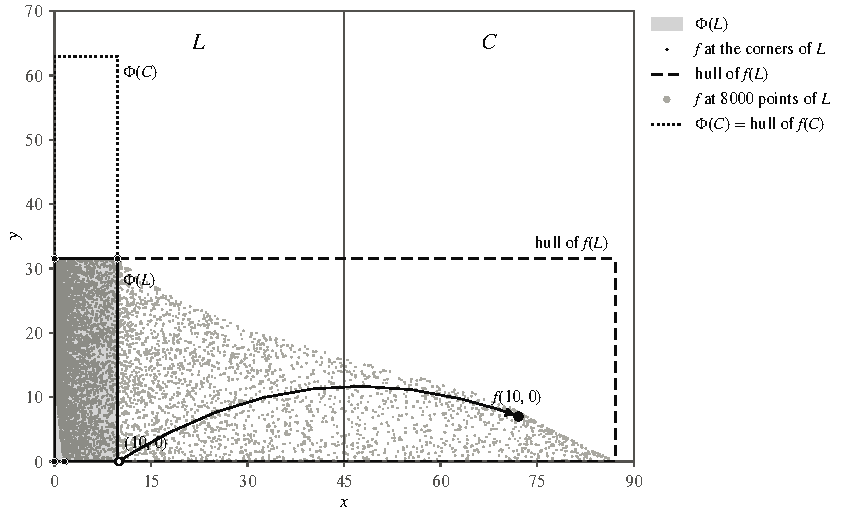
\includegraphics{leslie_depth_one.pdf}
\caption{The cells $L$ and $C$ of depth $1$. The box $\Phi(L)$ (gray) is spanned by $f$ at the four corners of $L$ (black dots), meets $L$ and lies in $x\leq9.80$. The box $\Phi(C)$ (dotted) is the hull of $f(C)$, since $f_1$ decreases in both variables on $C$, and lies in $L$. So the graph of the node of depth $1$ has only the edges $L\to L$ and $C\to L$, and $C$ is never refined. The hull of $f(L)$ (dashed) reaches $x=87.12$, and $f$ at $8000$ random points of $L$ (gray dots) covers a large part of $C$, for example $f(10,0)=(72.10,7.00)$.}\label{fig:levelone}
\end{figure}

Table~\ref{tab:chain} follows the boxes of depths $0$ to $12$ that contain $p=(7.7,16.9)$. The box of depth $12$ is the cell $c_p=[7.0303,8.4366]\times[16.4055,17.4992]$ of the Morse set $M$ of the run $12/14$ with $\Phi$ that contains $p^*$. The upper end of the $x$-range of $\Phi$ grows from $1.5117$ at depth $0$ to $86.3732$ at depth $6$ while the boxes shrink, and $\Phi(c_p)$ meets $C$, although $\Phi(L)$ does not.

\begin{table}[tbp]
\centering
\caption{The boxes $B$ of depths $0$ to $12$ that contain $p=(7.7,16.9)$, with the $x$-ranges of $\Phi(B)$ and $\hull f(B)$, whether $\Phi(B)$ lies in $\Phi$ of the parent of $B$, whether $f(B)\subseteq\Phi(B)$, and whether $\Phi(B)$ meets $C$ (computed, part 4 of \path{outputs/leslie_depth_one_cmgdb-1.5.3_fork.7.dev0-96642f2.txt}).}\label{tab:chain}
\footnotesize
\setlength{\tabcolsep}{4.5pt}
\begin{tabular}{rllllll}
\toprule
depth & $B$ & $\Phi(B)$ & $\hull f(B)$ & in parent & outer & meets $C$ \\
\midrule
0 & $[-0.0010,90.0000]\times[-0.0010,70.0000]$ & $[-0.0433,1.5117]$ & $[-0.0433,87.1154]$ & & no & no \\
1 & $[-0.0010,44.9995]\times[-0.0010,70.0000]$ & $[-0.0433,9.7992]$ & $[-0.0433,87.1154]$ & no & no & no \\
2 & $[-0.0010,44.9995]\times[-0.0010,34.9995]$ & $[-0.0433,25.0304]$ & $[-0.0433,87.1154]$ & no & no & no \\
3 & $[-0.0010,22.4992]\times[-0.0010,34.9995]$ & $[-0.0433,46.4851]$ & $[-0.0433,87.1154]$ & no & no & yes \\
4 & $[-0.0010,22.4992]\times[-0.0010,17.4992]$ & $[-0.0433,72.0180]$ & $[-0.0433,87.1154]$ & no & no & yes \\
5 & $[-0.0010,11.2491]\times[-0.0010,17.4992]$ & $[-0.0433,72.0180]$ & $[-0.0433,87.1154]$ & yes & no & yes \\
6 & $[-0.0010,11.2491]\times[8.7491,17.4992]$ & $[35.8225,86.3732]$ & $[35.8225,87.1154]$ & no & no & yes \\
7 & $[5.6241,11.2491]\times[8.7491,17.4992]$ & $[35.8225,75.4054]$ & $[35.8225,75.4054]$ & yes & yes & yes \\
8 & $[5.6241,11.2491]\times[13.1242,17.4992]$ & $[35.8225,64.5756]$ & $[35.8225,64.5756]$ & yes & yes & yes \\
9 & $[5.6241,8.4366]\times[13.1242,17.4992]$ & $[43.3365,64.5756]$ & $[43.3365,64.5756]$ & yes & yes & yes \\
10 & $[5.6241,8.4366]\times[15.3117,17.4992]$ & $[43.3365,58.2720]$ & $[43.3365,58.2720]$ & yes & yes & yes \\
11 & $[7.0303,8.4366]\times[15.3117,17.4992]$ & $[43.3365,53.5789]$ & $[43.3365,53.5789]$ & yes & yes & yes \\
12 & $[7.0303,8.4366]\times[16.4055,17.4992]$ & $[43.3365,50.5137]$ & $[43.3365,50.5137]$ & yes & yes & yes \\
\bottomrule
\end{tabular}
\end{table}

\subsection{The cycle through \texorpdfstring{$C$}{C} and the pair of \texorpdfstring{$M$}{M}}\label{sec:cycle}

On the final grid of the run $12/14$ with $\Phi$, which has $636$ cells, $M$ consists of $525$ cells of depth $12$. The set $X=\cover\Phi(M)$ has $534$ cells and contains $M$, and $A=X\setminus M$ has $9$ cells: eight cells of depths $8$ to $12$ in $[5.62,18.28]\times[4.37,13.12]$, which form a component $A_1$ of $|A|$, and $C$. The cells of $A_1$ map only into $C$. The cell $C$ maps into the six cells of $M$ that form $[1.4053,9.8429]\times[30.6244,31.7182]$ and into $12$ cells outside $X$, among them $C'$, and $28$ cells of $M$ map into $C$ (Figure~\ref{fig:cycle}). So $\cover\Phi(A)\cap X\not\subseteq A$, and $(X,A)$ is not a combinatorial index pair.

The map $f$ itself has both edges of the cycle $M\to C\to M$. The point $p=(7.7,16.9)\in c_p$ has $f(p)=(47.0842,5.3900)\in C$, and $q=(45.2,0.5)\in C$ has $f(q)=(9.2990,31.6400)$ in the cell $[8.4366,9.8429]\times[30.6244,31.7182]$ of $M$, in no cell of $A$ (computed, exact evaluations). Since $q\in|A|$ and $f(q)\in|X|\setminus|A|$, the pair $(|X|,|A|)$ violates (ii) of Definition~\ref{def:pair} for $f$. The condition also fails for the map that chomp lifts, which evaluates $\Phi$ on the boxes of depth $12$ in $C$: $23$ of these $2048$ boxes have images that meet $|M|$, all in $[45.000,46.406]\times[-0.001,25.156]$ (computed).

\begin{figure}[tbp]
\centering
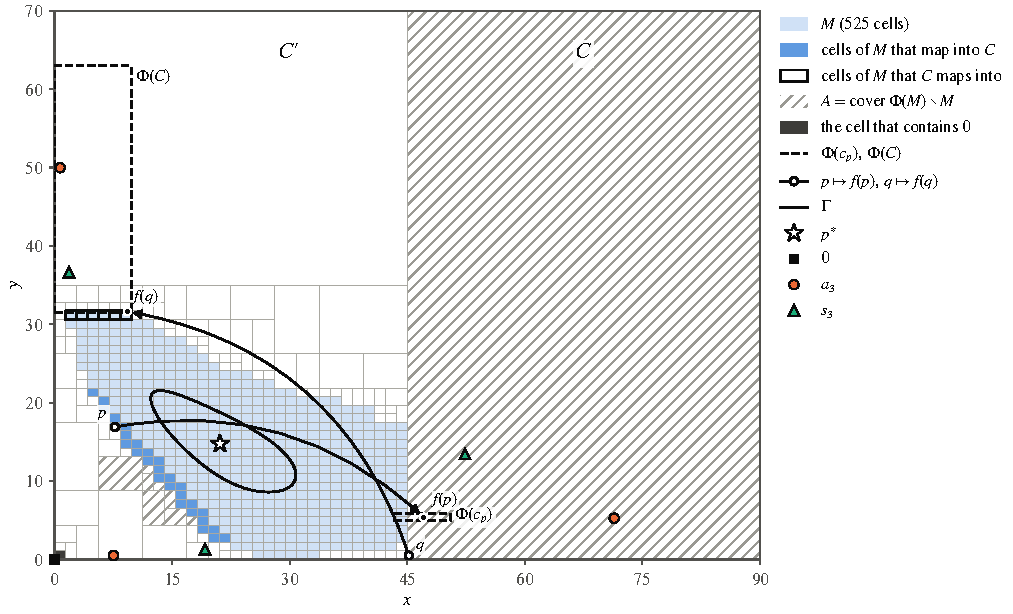
\includegraphics[width=\textwidth]{leslie_cycle_12_14.pdf}
\caption{The final grid of the run $12/14$ with $\Phi$ ($636$ cells) and the cycle $M\to C\to M$ (computed). $M$ (light blue, $525$ cells) is the Morse set that contains $p^*$. Its $28$ cells that map into $C$ are dark blue, and the $6$ cells that $C$ maps into are outlined in black. The hatched cells form $A=\cover\Phi(M)\setminus M$, eight small cells and $C$. $C'$ is the cell of depth $2$. The dashed boxes are $\Phi(c_p)$, for the cell $c_p$ of $M$ that contains $p=(7.7,16.9)$, and $\Phi(C)$. The arrows join $p$ to $f(p)=(47.08,5.39)\in C$ and $q=(45.2,0.5)\in C$ to $f(q)=(9.30,31.64)\in|M|$, so $f$ itself has both edges of the cycle.}\label{fig:cycle}
\end{figure}

The combinatorial analog of the inclusion $i$ of Section~\ref{sec:pairs}, with $\cover\Phi(A)$ in place of $f(P_0)$, fails to induce an isomorphism. The difference $(X\cup\cover\Phi(A))\setminus(A\cup\cover\Phi(A))=M\setminus\cover\Phi(A)$ has $519$ cells, not the $525$ cells of $M=X\setminus A$, and Table~\ref{tab:ranks} shows that the inclusion $(X,A)\to(X\cup\cover\Phi(A),A\cup\cover\Phi(A))$ induces no isomorphism in degree $1$, where the ranks are $1$ and $2$. So the combinatorial analog of the index map $i_*^{-1}\circ f_*$ is not defined for this pair. That $(|X|,|A|)$ is not an index pair for $f$ rests on the point $q$ above.

\begin{table}[tbp]
\centering
\caption{Ranks of the homology over $\F$ in degrees $0$, $1$, $2$ of the unions of cells, from the cubical chain complexes at depth $12$ (computed, exact linear algebra modulo $5$, part 4 of \path{outputs/leslie_cycle_cmgdb-1.5.3_fork.7.dev0-96642f2.txt}). Here $\cover\Phi(A)$ has $19$ cells.}\label{tab:ranks}
\begin{tabular}{lrl}
\toprule
space & cells & ranks \\
\midrule
$X$ & $534$ & $(1,0,0)$ \\
$A$ & $9$ & $(2,0,0)$ \\
$(X,A)$ & & $(0,1,0)$ \\
$X\cup\cover\Phi(A)$ & $546$ & $(1,1,0)$ \\
$A\cup\cover\Phi(A)$ & $27$ & $(2,0,0)$ \\
$(X\cup\cover\Phi(A),A\cup\cover\Phi(A))$ & & $(0,2,0)$ \\
\bottomrule
\end{tabular}
\end{table}

\code{ComputeConleyMorseGraph} annotates $M$ with $(0,x+1,0)$ on all four builds. This annotation has the ranks of $H_*(X,A)=(0,\F,0)$, and chomp computed an endomorphism of $H_1(X,A)$ whose invertible part is $-1$, outside the assumptions of its lift. Which step of the lift produces $-1$ was not traced. If $(X,A)$ were an index pair, $(0,x+1,0)$ would be, for example, the annotation of the index of a hyperbolic fixed point with a one-dimensional unstable direction and an unstable eigenvalue below $-1$, and no fixed point of $f$ is of this kind (Proposition~\ref{prop:fixed}).

The set $M$ is a strongly connected component of the graph of its node of depth $12$, whose grid does not contain $C$, and not of the graph of the final grid. The component $N$ of the graph of the final grid that contains $M$ has $612$ cells, among them $41$ cells of depth less than $12$, $C$, $C'$, the cell of the origin and the points of $a_3$ and $s_3$. Its pair is $(N,\emptyset)$ since $\cover\Phi(N)=N$, and \code{ComputeConleyIndexForCells} returns $(x-1,0,0)$ for it on all four builds. The box $\Phi(c)$ misses part of $f(c)$ for four of its cells, so $(|N|,\emptyset)$ is not known to be an index pair for $f$ (computed).

\begin{table}[tbp]
\centering
\caption{The set $M$ of the run $12/14$ with $\Phi$ on each build (computed, \path{outputs/leslie_before_after.txt}). The message of master continues ``cell 635 of A maps into cell 177 of S (cells of A that map into X \textbackslash{} A: 1 of 9)''. Cell $635$ is $C$.}\label{tab:builds}
\begin{tabular}{lll}
\toprule
build & annotation of $M$ & \code{ComputeConleyIndexForCells}$(M)$ \\
\midrule
upstream 1.5.2 & $(0,x+1,0)$ & $(0,x+1,0)$ \\
1.3.3+fork.6 & $(0,x+1,0)$ & $(0,x+1,0)$ \\
0e21503 & $(0,x+1,0)$ & $(0,x+1,0)$ \\
master 96642f2 & $(0,x+1,0)$ & \code{ValueError}, ``the cells S do not give an index pair'' \\
\bottomrule
\end{tabular}
\end{table}

Table~\ref{tab:builds} compares the builds. Since commit 86b143a, ``Refuse cell sets that give no index pair in \code{ComputeConleyIndexForCells}'', this function checks the condition $\cover F(A)\cap X\subseteq A$ on the cells and raises \code{ValueError} when it fails. The commit does not change the hierarchy, and \code{ComputeConleyMorseGraph} returns the same annotations as before.

\subsection{The invariant set in \texorpdfstring{$|M|$}{|M|}}\label{sec:isolation}

Let $M_{12}=M$ and let $M_{16}$ be the Morse set that contains $p^*$ in the run $16/18$ with $\Phi$.

\begin{proposition}\label{prop:isolation}
Let $\mathcal{G}$ be the graph on the boxes of depth $16$ in $|M_{12}|$ with an edge $c\to c'$ when $\Phihull(c)\cap c'\neq\emptyset$, and suppose that
\begin{enumerate}[label=(\alph*)]
\item the boxes on paths of $\mathcal{G}$ that are infinite in both directions are the cells of $M_{16}$, and $|M_{16}|\subseteq\interior|M_{12}|$,
\item $\Phihull(c)\subseteq\interior|M_{16}|$ for every cell $c$ of $M_{16}$, and
\item $|M_{16}|$ is connected and $H_1(|M_{16}|;\F)=0$.
\end{enumerate}
Then $K_{16}=\bigcap_{n\geq0}f^n(|M_{16}|)$ is an attractor, $\Inv(|M_{12}|)=K_{16}$, and the Conley index of $K_{16}$ has the annotation $(x-1,0,0)$. In particular, $(0,x+1,0)$ is not the annotation of the Conley index of $\Inv(|M_{12}|)$.
\end{proposition}

\begin{proof}
Since $f(c)\subseteq\Phihull(c)$ by Lemma~\ref{lem:hull}, the boxes of depth $16$ that contain the points of an orbit of $f$ in $|M_{12}|$ form a path of $\mathcal{G}$ that is infinite in both directions. By (a), $\Inv(|M_{12}|)\subseteq|M_{16}|\subseteq\interior|M_{12}|$. By (b), $f(|M_{16}|)\subseteq\interior|M_{16}|$, so $K_{16}$ is an attractor, $f(K_{16})=K_{16}$, $K_{16}=\Inv(|M_{16}|)$, and $(|M_{16}|,\emptyset)$ is an index pair for $K_{16}$. As an invariant subset of $|M_{12}|$, $K_{16}$ lies in $\Inv(|M_{12}|)$, and as an invariant subset of $|M_{16}|$, $\Inv(|M_{12}|)$ lies in $K_{16}$. By (c), $H_*(|M_{16}|;\F)$ is $\F$ in degree $0$, on which $f$ induces the identity. The last statement follows, since annotations are invariants of the Conley index (Section~\ref{sec:annotations}).
\end{proof}

The hypotheses hold in a double precision computation with margins (\path{leslie_isolation.py}, computed). The boxes on paths of $\mathcal{G}$ infinite in both directions are the $5570$ cells of $M_{16}$, among the $8400$ boxes of depth $16$ in $|M_{12}|$, and at least two boxes separate them from the boxes outside $|M_{12}|$. For every cell $c$ of $M_{16}$, $\Phihull(c)$ stays at distance at least $2.327\times10^{-5}$ from the boxes outside $M_{16}$. With the widening $10^{-6}$ in place of $10^{-9}$, the same holds with the margin $6.067\times10^{-6}$, and with the widening $10^{-4}$ the set of boxes changes, to $5588$ boxes. The Betti numbers of $|M_{16}|$ and $|M_{12}|$ are $(1,0,0)$. Since $|M_{12}|$ contains no point of $0$, $a_3$ or $s_3$, and the simulations find no other invariant set there, we infer that $K_{16}=K$, the disk bounded by $\Gamma$.

So the runs $12/14$ and $16/18$ isolate the same attractor and annotate it differently. The set $|M_{12}|$ isolates $K_{16}$, inferred to be $K$, but it is not an attracting block, since $p\in c_p\subseteq|M_{12}|$ and $f(p)\in C$ lies outside $|M_{12}|$ (Section~\ref{sec:cycle}). The hulls illustrate this: $\Phihull(c)$ meets a cell outside $M_{12}$ for $46$ of its $525$ cells, $28$ of them in $C$, and meets a box outside $|M_{12}|$ for $382$ of its $8400$ boxes of depth $16$. The set $M_{16}$ has the same $5570$ boxes as the Morse set around $p^*$ of the uniform run of depth $16$, and $\cover\Phi(M_{16})=M_{16}$, so $C$ never enters its pair.

\subsection{Monotonicity under refinement}\label{sec:monotone}

\begin{lemma}\label{lem:monotone}
Let $G$ be the graph of the final grid of $\mathrm{Model}(\dmin,\dmax,\dinit,\mathit{limit},Q,F)$, and suppose that $F$ is monotone under refinement. Then
\begin{enumerate}[label=(\arabic*)]
\item no cell of depth less than $\dmin$ lies on a cycle of $G$, and
\item the strongly connected components of $G$ that contain a cycle are the Morse sets of the Morse graph.
\end{enumerate}
\end{lemma}

\begin{proof}
Our strategy is to project a cycle of $G$ to each depth $j\geq\dinit$ and to follow the projection through the nodes of the hierarchy. For a cell $c$ of $G$ and $\dinit\leq j<\depth(c)$, the hierarchy bisected each of the boxes $\pi_j(c),\pi_{j+1}(c),\dots$ that contain $c$ strictly, so iterating the inclusion $F(b)\subseteq F(B)$ of Section~\ref{sec:boxmaps} yields
\[
F(c)\subseteq F(\pi_j(c)).
\]
Since $c'\subseteq\pi_j(c')$, an edge $c\to c'$ of $G$ yields $F(\pi_j(c))\cap\pi_j(c')\neq\emptyset$.

Let $c_0\to c_1\to\dots\to c_m=c_0$ be a cycle of $G$. We show by induction on $j=\dinit,\dots,\dmin$ that there is a node $N_j$ of depth $j$ whose grid contains all $\pi_j(c_i)$. For $j=\dinit$ this holds for the root. Given $N_j$, the boxes $\pi_j(c_0),\dots,\pi_j(c_m)$ form a closed walk in the graph of $N_j$, which uses the same $F$ on the same cells, so they lie in one Morse set $S_j$ of $N_j$. If $j<\dmin$, then $S_j$ has a child $N_{j+1}$, whose grid consists of the halves of the cells of $S_j$, and the grid of $N_{j+1}$ enters the final grid. So no cell of $S_j$ is a cell of $G$, $\depth(c_i)>j$, and $\pi_{j+1}(c_i)$ is a half of $\pi_j(c_i)$, a cell of the grid of $N_{j+1}$. This completes the induction and proves (1).

For (2), let $S$ be the Morse set of $N_{\dmin}$ that contains all $\pi_{\dmin}(c_i)$. If $S$ is a vertex of the Morse graph, then neither $N_{\dmin}$ nor the child of $S$ is discarded, no grid deeper than $\dmin$ refines $S$ in the final grid, and $c_i=\pi_{\dmin}(c_i)\in S$. Suppose that $S$ is not a vertex. A node with a Morse set is discarded only if it has children and all of them are discarded, so in either case $S$ has a child $N'$, and $N'$ is discarded. The grid of $N'$, refined by the grids of its descendants, enters the final grid, so the induction step applies to $N'$ and continues node by node through discarded nodes below depth $\dmin$. Since the depth is at most $\dmax$, it ends at a discarded node without children, which has no Morse set, although its graph contains the closed walk of the projections. This contradiction shows that every cycle of $G$ lies in a Morse set of the Morse graph, and hence so does every strongly connected component of $G$ that contains a cycle. Conversely, a Morse set $S$ of the Morse graph is strongly connected in the graph of its node, its cells are cells of $G$, and the edges between them are edges of $G$. So $S$ lies in one strongly connected component of $G$, which contains a cycle and therefore lies in $S$.
\end{proof}

The lemma needs no outer approximation. An outer approximation is what makes the Morse sets isolating neighborhoods for $f$.

\begin{corollary}\label{cor:outer}
Under the hypothesis of Lemma~\ref{lem:monotone}, $(\cover F(S),\cover F(S)\setminus S)$ is a combinatorial index pair on the final grid for every Morse set $S$ of the Morse graph. If $F$ is moreover an outer approximation of $f$, then $\Inv(|S|)$ lies in the interior of $|S|$ relative to $Q$.
\end{corollary}

\begin{proof}
By Lemma~\ref{lem:monotone}(2), $S$ is a strongly connected component of $G$, so every cell on a path of $G$ between two cells of $S$ belongs to $S$, and Lemma~\ref{lem:pair} applies. Let $x\in\Inv(|S|)$, and suppose that $x$ lies in a cell $c'\notin S$. A full orbit of $x$ in $|S|$ has points $x_{-1}$ and $f(x)$ with $f(x_{-1})=x$, which lie in cells $b,e\in S$. Since $f(b)\subseteq F(b)$ and $f(c')\subseteq F(c')$, $G$ has the edges $b\to c'\to e$, so $c'\in S$, a contradiction. Hence $\Inv(|S|)$ lies in no cell outside $S$.
\end{proof}

For $\Phi$ on the Leslie map, the hypothesis fails along the chain of $c_p$ at depths $1$, $2$, $3$, $4$ and $6$ (Table~\ref{tab:chain}), and $\Phi(c_p)\not\subseteq\Phi(L)$. The cycle $M\to C\to M$ projects at depth $1$ to $L\to C\to L$, but $L\to C$ is not an edge of the graph of the node of depth $1$.

Table~\ref{tab:boxes} tests both properties on every box that the hierarchy evaluates. The box map is wrapped so that every call of \code{ComputeMorseGraph}, in the hierarchy and in the final map graph, is logged, and each distinct box $B$ of depth $d\geq1$ is compared with its parent $B'$. The hierarchy evaluates more boxes than the cells of the final grid and their ancestors. By Section~\ref{sec:hierarchy}, the child of a Morse set $S$ of depth $j\geq\dmin$ is decomposed if $j<\dmax$ and its grid, with $2|S|$ cells, has at most $\mathit{limit}=10000$ cells, and these decompositions decide which nodes are discarded. For example, $2904$ of the $4175$ boxes of the run $12/14$ with $\Phi$ have depth $13$ or $14$. In the run $16/18$ with $\Phi$, the child of $M_{16}$ has $11140$ cells and is not decomposed, and the $4$ boxes deeper than $16$ come from the cell of the origin. For $\Phi$, $\hull f(B)$ sticks out of $\Phi(B)$ by up to $0.971$ and $\Phi(B)$ out of $\Phi(B')$ by up to $0.469$, relative to $1+m$ with $m$ the largest absolute value of an end, and neither happens at depth $10$ or more. For $\Phipad$, the largest such excess of $\Phipad(B)$ over $\Phipad(B')$ at depth $10$ or more is $4.81\times10^{-3}$. Counting every positive excess yields the same numbers as the threshold $10^{-8}$ of the table.

\begin{table}[tbp]
\centering
\caption{Outer approximation and monotonicity on the boxes that the hierarchy evaluates, with the threshold $10^{-8}$ relative to $1+m$ (computed, \path{outputs/leslie_monotonicity_cmgdb-1.5.3_fork.7.dev0-96642f2.txt}, with the depths of the grids and the last column from \path{outputs/leslie_morse_cmgdb-1.5.3_fork.7.dev0-96642f2.txt}). For each run: the cells of the final grid and the depth of the coarsest one, the distinct boxes evaluated and those deeper than $\dmin$, the boxes with $\hull f(B)\not\subseteq F(B)$ and with $F(B)\not\subseteq F(B')$ for the parent $B'$, with their depths, and the cells of depth less than $\dmin$ on cycles of the graph of the final grid. The distinct boxes and the failures are the same on all four builds.}\label{tab:boxes}
\small
\begin{tabular}{llllll}
\toprule
run & final grid & boxes & not outer & not monotone & on cycles \\
\midrule
$\Phi$, $12/14$ & $636$, from $1$ & $4175$ ($2904$) & $15$, depths $0$ to $9$ & $10$, depths $1,2,3,4,6$ & $41$ \\
$\Phi$, $16/18$ & $7059$, from $1$ & $14121$ ($4$) & $15$, depths $0$ to $9$ & $10$, depths $1,2,3,4,6$ & $446$ \\
$\Phipad$, $12/14$ & $1473$, from $4$ & $9203$ ($6258$) & $4$, depths $1,2,3,5$ & $24$, even depths $2$ to $14$ & $0$ \\
$\Phipad$, $16/18$ & $14151$, from $4$ & $31909$ ($3608$) & $4$, depths $1,2,3,5$ & $44$, even depths $2$ to $18$ & $0$ \\
$\Phihull$, $12/14$ & $1073$, from $2$ & $6255$ ($4110$) & $0$ & $0$ & $0$ \\
$\Phihull$, $16/18$ & $8759$, from $2$ & $18533$ ($1044$) & $0$ & $0$ & $0$ \\
\bottomrule
\end{tabular}
\end{table}

\subsection{Three box maps compared}\label{sec:compare}

By Lemma~\ref{lem:hull}, the box $\hull f(B)$, which $\Phihull$ computes in floating point, is an outer approximation of $f$, and the widening of $\Phihull$ is meant to cover the rounding of $f$. The test of Table~\ref{tab:boxes} compares $\Phihull$ with itself, so the closed form was also checked against $f$ by sampling, and the check agrees with this: on $3000$ random boxes with widths from $10^{-3}$ to $10^{2}$, no value of $f_1$ at a $60\times60$ grid of points and at $2000$ points of each edge exceeds the hull, and the hull exceeds the largest sampled value by at most $1.4\times10^{-6}$, relative (computed). $\Phihull$ is monotone under refinement, since $f(b)\subseteq f(B)$ implies $\hull f(b)\subseteq\hull f(B)$, and the widening does not decrease from $b$ to $B$. So Lemma~\ref{lem:monotone} applies to $\Phihull$, and Corollary~\ref{cor:outer} applies up to the rounding of $f$. The runs with $\Phihull$ refine $C$ at depth $2$, have no cell of depth less than $\dmin$ on a cycle, and have Morse sets equal to the strongly connected components of the graph of the final grid that contain a cycle (computed). Their annotations equal \code{ComputeConleyIndexForCells} for every Morse set. The final grid of the run $16/18$ has $28$ cells of depth $17$, from a child that the hierarchy discarded.

Padding removes the failure on the Leslie map because $\Phipad(L)$, with $x$-range $[-45.0438,54.7997]$, happens to reach $C$. It is not an outer approximation, since $f_1$ reaches $87.1154$ on $L$, and it is not monotone under refinement (Table~\ref{tab:boxes}). Still, the runs with $\Phipad$ satisfy the conclusions of Lemma~\ref{lem:monotone}. Their run $16/18$ puts $s_3$ and $K$ into one Morse set, annotated $(0,x^2+x+1,0)$, the annotation of the index of $J$ (Proposition~\ref{prop:J}).

With $\Phi$, the run $16/18$ also violates the conclusions of Lemma~\ref{lem:monotone}: $446$ cells of depth less than $16$ lie on cycles, in a component of $472$ cells of depths $1$ to $16$ that contains the cell of the origin, $C$, $C'$, $a_3$ and $s_3$. Its annotations come from valid pairs nevertheless: $\cover\Phi(M_{16})=M_{16}$, and the pair of the cell of the origin, with $|X|=7$ and $|A|=6$, is a combinatorial index pair, although that cell is not a strongly connected component of the graph of the final grid.

\subsection{The origin}\label{sec:origin}

The Morse set that contains $0$ is annotated $(0,0,0)$ in every run on $Q$. Since $0\in\interior Q$, the index of $\{0\}$ for $f$ on $Q$ is that of the saddle, with the annotation $(0,x-1,0)$ (Table~\ref{tab:expected}). In every run, this Morse set is the cell of $0$, which has the corner $(-0.001,-0.001)$ since the cells are wider than the distance $0.001$ from $0$ to $\partial Q$, and $f$ maps part of this cell out of $Q$. For example, $(-0.0009,0)$ lies in the interior of the cell, and $f(-0.0009,0)=(-0.017642,-0.00063)$ lies outside $Q$. Along the unstable direction, the points $-t(1,0.034293)$ lie in $Q$ only for $t\leq0.001$, and the branch of $W^u(0)$ tangent to them escapes: all $200$ points of a fundamental domain of that branch reach $x<-1000$ within $50$ steps (computed). CMGDB discards the parts of the images outside $Q$, which meet no cell, so no cell of $X$ carries this exit, and $(|X|,|A|)$ violates (iii) of Definition~\ref{def:pair} at $(-0.0009,0)$. Hence $(|X|,|A|)$ is not an index pair for $f$, and its annotation $(0,0,0)$ differs from that of the index of $\{0\}$. Reading the clipped images as images of $\rho_Q\circ f$, where $\rho_Q$ clamps each coordinate to $Q$, does not help: since $f(-0.001,-0.0007)=(-0.036182,-0.0007)$, the point $(-0.001,-0.0007)$ of the same cell is a fixed point of $\rho_Q\circ f$, so the invariant set of $\rho_Q\circ f$ in the cell is larger than $\{0\}$. Table~\ref{tab:origin} varies the domain.

\begin{table}[tbp]
\centering
\caption{The Morse set that contains $0$, with $\Phi$ at uniform depth $14$, on six domains $[x_0,90]\times[y_0,70]$ (computed, \path{outputs/leslie_origin_cmgdb-1.5.3_fork.7.dev0-96642f2.txt}). Here $t_{\max}$ is the largest $t$ with $-t(1,0.034293)$ in the domain, and the sixth column is the number of cells of the exit set $A$ whose interiors meet the segment $\{-t(1,0.034293):0<t<t_{\max}\}$. \code{ComputeConleyIndexForCells} equals the annotation in every row, on all four builds.}\label{tab:origin}
\small
\setlength{\tabcolsep}{4pt}
\begin{tabular}{lllllll}
\toprule
$(x_0,y_0)$ & $t_{\max}$ & cells & \begin{tabular}[b]{@{}l@{}}touches the\\boundary\end{tabular} & exit set $A$ & \begin{tabular}[b]{@{}l@{}}cells of $A$ on\\the segment\end{tabular} & annotation \\
\midrule
$(-0.001,-0.001)$ & $0.001$ & $1$ & yes & $33$ cells, $1$ component & $0$ & $(0,0,0)$ \\
$(-0.001,-1)$ & $0.001$ & $1$ & yes & $43$ cells, $1$ component & $0$ & $(0,0,0)$ \\
$(-1,-0.001)$ & $0.029$ & $1$ & yes & $28$ cells, $2$ components & $0$ & $(0,0,0)$ \\
$(-1,-0.05)$ & $1$ & $1$ & yes & $27$ cells, $2$ components & $1$ & $(0,x-1,0)$ \\
$(-1,-1)$ & $1$ & $7$ & yes & $156$ cells, $2$ components & $1$ & $(0,x-1,0)$ \\
$(-5,-5)$ & $5$ & $14$ & no & $261$ cells, $2$ components & $6$ & $(0,x-1,0)$ \\
\bottomrule
\end{tabular}
\end{table}

The annotation is $(0,x-1,0)$ exactly in the rows of Table~\ref{tab:origin} in which the segment $\{-t(1,0.034293):0<t<t_{\max}\}$ meets a cell of the exit set, and $(0,0,0)$ in the rows in which it stays in the cell of $0$ (computed). On $[-5,90]\times[-5,70]$, the Morse set has $14$ cells in $[-2.773,3.164]\times[-2.070,2.031]$, away from the boundary. The domains $[-1,90]\times[-0.001,70]$ and $[-1,90]\times[-0.05,70]$ form a controlled comparison. In both, the points $t(1,-0.861996)$ with $t\geq0$ leave the domain inside the cell of the origin, at $t=0.00116$ and $t=0.058$, and both domains contain $-t(1,-0.861996)$ for $0\leq t\leq1$. They differ along the unstable direction: $-t(1,0.034293)$ lies in the first domain only for $t\leq0.029$, inside the cell of the origin, and in the second for $t\leq1$, through the cell $[-1,-0.289]\times[-0.05,0.497]$ of the exit set. The annotations are $(0,0,0)$ and $(0,x-1,0)$. That the difference along the unstable direction causes the different annotations, and that the stable direction plays no role, is inferred from these runs. In every row, $f$ maps points of the cell of $0$ out of the domain (computed), so no row yields an index pair for $f$, and the agreement of the last three rows with the annotation of the index of $\{0\}$ is an observation, not a consequence of Definition~\ref{def:pair}.

On $Q$, in the run $12/14$ with $\Phi$, the pair of the cell of the origin is a combinatorial index pair with $|X|=22$ and $|A|=21$, in one component of depths $7$ to $12$, and $H_*(X,A;\F)=0$, which forces the annotation $(0,0,0)$ (computed). So the trivial annotation on $Q$ is a limitation of how CMGDB treats images that leave $Q$, not a property of the index of $\{0\}$, and it is unrelated to the defect of this part, since the uniform runs show it too.

\subsection{The builds}\label{sec:lesliebuilds}

On the four builds, every grid, Morse set, annotation, Morse graph edge, pair check and strongly connected component of the Leslie runs agrees, and so do the results of \path{leslie_depth_one.py}, \path{leslie_isolation.py} and \path{leslie_origin.py} and every distinct evaluated box and failure count of \path{leslie_monotonicity.py} (computed, with the boxes compared through SHA-256 digests). The only difference in results is \code{ComputeConleyIndexForCells}$(M)$ for the run $12/14$ (Table~\ref{tab:builds}). Upstream 1.5.2 calls the box map fewer times, for example $4175$ times against $4811$ for the run $12/14$ with $\Phi$, and the differences equal the sizes of the final grids. The fork builds evaluate the final grid once more to cache the map graph that they return, which upstream computes lazily, and this explanation is inferred from the documented defaults. The defect of Part I does not change any Leslie result: the Morse sets of the run $16/18$ with $\Phihull$ whose pairs contain cells of depth $17$ have the same annotations on all builds.

\section{Consequences for using CMGDB}\label{sec:consequences}

The defect of Part I affects builds before commit 577d988, among them upstream 1.5.2, the fork release 1.3.3+fork.6 and the merge 0e21503, on runs with $\dmax>\dmin$ (Corollary~\ref{cor:scope}). A Morse set is affected when $X=\cover F(S)$ contains a cell deeper than $S$ whose ancestor at the depth of $S$ sticks out of the hull of the cells of $X$. In the examples these cells appear to come from refined and discarded neighbors of hyperbolic fixed points (Section~\ref{sec:scope}), and the annotations were trivial or undefined, or the fork release 1.3.3+fork.6 raised \code{RuntimeError} and returned no annotation. A run shows the defect when its box map receives, during \code{ComputeConleyMorseGraph}, a box that is not a box of the bisection tree. The regression tests check this by wrapping the box map, and a user can do the same. On the old builds, $\dmax=\dmin$ avoids the defect for any $\dinit$. Master 96642f2 bounds the complex by its cubes, and on the examples it returns the indices of the linearization. It does not check that the cubical pair $(X',A')$ is an index pair for $\Fc$ (Section~\ref{sec:fix}).

The defect of Part II affects hierarchical runs, $\dinit<\dmin$, with a box map that is not monotone under refinement, on every build including master. \code{CMGDB.BoxMap(f, B)} with its default \code{padding=False} spans $f$ at the corners of $B$, and it can be such a box map when a coordinate of $f$ is not monotone on the coarse boxes, as for the Leslie map. \code{ComputeConleyMorseGraph} then annotates Morse sets whose pairs are not index pairs, without a warning. Two checks are available on master. \code{ComputeConleyIndexForCells(model, morse\_graph, morse\_graph.morse\_set(v))} raises \code{ValueError} when the pair of the Morse set $v$ is not a combinatorial index pair. The conclusions of Lemma~\ref{lem:monotone} can be tested on the map graph that \code{ComputeConleyMorseGraph} returns: the strongly connected components of the graph of the final grid that contain a cycle should be the Morse sets, and no cell of depth less than $\dmin$ should lie on a cycle. These checks concern the cells and do not certify isolation for $f$. To avoid the defect, use a box map that is an outer approximation of $f$ and monotone under refinement, for example the hull of $f(B)$ when it can be computed, as for the Leslie map, or an interval enclosure, which is monotone under inclusion. By Lemma~\ref{lem:monotone} and Corollary~\ref{cor:outer}, the Morse sets are then the strongly connected components of the graph of the final grid, their pairs are combinatorial index pairs, and they are isolating neighborhoods for $f$. Uniform runs, $\dinit=\dmin=\dmax$, avoid the hierarchy altogether: their Morse sets are strongly connected components of the graph of the final grid, so their pairs are combinatorial index pairs by Lemma~\ref{lem:pair}, although isolation for $f$ still needs an outer approximation. Padding removed the failure on the Leslie map, but it is neither an outer approximation nor monotone under refinement there.

Finally, CMGDB discards the parts of the images that leave $Q$. If $f$ maps points of a Morse set $S$ out of $Q$, the pair of $S$ is not an index pair for $f$, and its annotation can differ from that of the index of the invariant set, even when that set lies in $\interior Q$. At the origin of the Leslie map, whose cell reaches $\partial Q$, the annotation is $(0,0,0)$ and the index has the annotation $(0,x-1,0)$ (Section~\ref{sec:origin}). This is a limitation of how CMGDB treats images that leave $Q$, not a property of the index, and it affects every build. If $F$ is an outer approximation of $f$ and $F(c)\subseteq Q$ for every cell $c$ of $S$, then $f(|S|)\subseteq|X|$, and this failure cannot occur. On the domains of Table~\ref{tab:origin}, the annotation of the origin agrees with that of its index exactly when the segment $\{-t(1,0.034293):0<t<t_{\max}\}$ meets a cell of the exit set, although $f$ maps points of the cell of the origin out of the domain on all of them.

\section{Reproduction}\label{sec:reproduction}

The scripts are in \path{scripts/}, their outputs in \path{outputs/} and the figures in \path{figures/}, next to this report. \path{README.md} lists the environments, the commands, the script that regenerates each table and figure, and the runtimes. Each script that uses CMGDB runs on any of the four builds, and the names of its outputs end with a tag of the build, \path{cmgdb-1.5.2}, \path{cmgdb-1.3.3_fork.6}, \path{cmgdb-1.5.3_fork.7.dev0-0e21503} or \path{cmgdb-1.5.3_fork.7.dev0-96642f2}, since the last two builds report the same version. The builds can be installed with
\needspace{8\baselineskip}
\begin{lstlisting}[language=bash,numbers=none]
pip install CMGDB==1.5.2
pip install cmgdb==1.3.3+fork.6 --find-links \
  https://github.com/bernardorivas/CMGDB/releases/expanded_assets/v1.3.3%2Bfork.6
pip install git+https://github.com/bernardorivas/CMGDB@0e21503
pip install git+https://github.com/bernardorivas/CMGDB@96642f2
\end{lstlisting}
in one Python 3.13 environment each, with numpy, matplotlib and pytest. The last two are built from source. 0e21503 needs a C++20 compiler and 96642f2 a C++17 compiler, and both need Boost with the chrono, thread and serialization libraries. The stored outputs assume that no \code{CMGDB\_MAPGRAPH\_*} variable is set, since \code{CMGDB\_MAPGRAPH\_CACHE} changes the counts of evaluations of $F$.

Part I: \path{bounds_annotations.py} computes the annotations (Table~\ref{tab:annotations}, with \path{--boxmap} for the runs with \code{CMGDB.BoxMap}), \path{bounds_references.py} the conditions of Lemma~\ref{lem:linear} and the uniform runs, \path{bounds_mechanism.py} the complexes, the boxes received by $F$, the maps on cubes and the lift on the line (Tables~\ref{tab:complexes} and~\ref{tab:e1}), \path{bounds_table.py} the tables across builds (Tables~\ref{tab:annotations} to~\ref{tab:complexes}), \path{bounds_figures.py} Figures~\ref{fig:e1line} to~\ref{fig:e4}, and \path{bounds_regression_tests.py} runs the regression tests. \path{bounds_run_all.py} runs all of them on several builds.

Part II: \path{leslie_dynamics.py} computes the dynamics of Section~\ref{sec:dynamics}, \path{leslie_morse.py} the Morse decompositions (Table~\ref{tab:morse}), \path{leslie_depth_one.py} the first depths and the chain of boxes (Table~\ref{tab:chain}), \path{leslie_cycle.py} the cycle, the pair and its homology (Tables~\ref{tab:ranks} and~\ref{tab:builds}), \path{leslie_isolation.py} the hypotheses of Proposition~\ref{prop:isolation}, \path{leslie_monotonicity.py} Table~\ref{tab:boxes}, \path{leslie_origin.py} Table~\ref{tab:origin}, and \path{leslie_before_after.py} the comparison of the builds. The four scripts \path{leslie_fig_*.py} draw Figures~\ref{fig:phase} to~\ref{fig:cycle}, and \path{leslie_run_all.py} runs everything.

\needspace{17\baselineskip}
Two short programs show the defects directly. The first is E1. On 1.5.2, 1.3.3+fork.6 and 0e21503 it prints the annotation \code{[\textquotesingle{}0\textquotesingle{}, \textquotesingle{}0\textquotesingle{}]} for the Morse set $[0.9375,1.015625]$, and on 96642f2 \code{[\textquotesingle{}0\textquotesingle{}, \textquotesingle{}x-1\textquotesingle{}]}.
\begin{lstlisting}[language=Python,numbers=none]
import CMGDB

def F(rect):
    # f(x) = x/(2 - x) is increasing, so f([a, b]) = [f(a), f(b)]
    return [t / (2.0 - t) for t in rect]

model = CMGDB.Model(4, 8, 0, 10000, [0.0], [1.25], F)
morse_graph, map_graph = CMGDB.ComputeConleyMorseGraph(model)
for v in range(morse_graph.num_vertices()):
    print(morse_graph.morse_set_boxes(v), morse_graph.annotations(v))
\end{lstlisting}
The second is the Leslie run $12/14$ with $\Phi$. On every build it prints \code{0 525 [\textquotesingle{}0\textquotesingle{}, \textquotesingle{}x+1\textquotesingle{}, \textquotesingle{}0\textquotesingle{}]} for vertex $0$ of the Morse graph, the Morse set $M$ of Section~\ref{sec:cycle}. \code{ComputeConleyIndexForCells} returns \code{[\textquotesingle{}0\textquotesingle{}, \textquotesingle{}x+1\textquotesingle{}, \textquotesingle{}0\textquotesingle{}]} on 1.5.2, 1.3.3+fork.6 and 0e21503 and raises \code{ValueError} on 96642f2.
\begin{lstlisting}[language=Python,numbers=none]
import math
import CMGDB

def f(x):
    s = x[0] + x[1]
    return [(19.6 * x[0] + 23.68 * x[1]) * math.exp(-0.1 * s), 0.7 * x[0]]

def F(rect):
    return CMGDB.BoxMap(f, rect)  # f at the corners of rect, no padding

model = CMGDB.Model(12, 14, [-0.001, -0.001], [90.0, 70.0], F)
morse_graph, map_graph = CMGDB.ComputeConleyMorseGraph(model)
for v in range(morse_graph.num_vertices()):
    print(v, len(morse_graph.morse_set(v)), morse_graph.annotations(v))
try:
    print(CMGDB.ComputeConleyIndexForCells(model, morse_graph, morse_graph.morse_set(0)))
except ValueError as error:
    print("ValueError:", str(error)[:72])
\end{lstlisting}

\begin{thebibliography}{9}

\bibitem{FR00}
J.~Franks and D.~Richeson, Shift equivalence and the Conley index, Trans. Amer. Math. Soc. 352 (2000), 3305--3322.

\bibitem{Mro99}
M.~Mrozek, An algorithmic approach to the Conley index theory, J. Dynam. Differential Equations 11 (1999), 711--734.

\end{thebibliography}

\end{document}
